% Feature Selection Chapter
% This chapter assumes the following directory structure:
% report/
%   ├── feature_selection.tex (this file)
%   ├── figures/              (correlation matrices and pairplots)
%   └── logs/                 (TopFeaturesTable.tex, FeatureSelectionCommands.tex, and other outputs)
%
% Run the Python feature selection script first to generate all required files

% Include the automatically generated commands
% Feature Selection LaTeX Commands - iBudget
% Generated: 2025-10-09 20:25:43
% Include with: % Feature Selection LaTeX Commands - iBudget
% Generated: 2025-10-09 20:25:43
% Include with: % Feature Selection LaTeX Commands - iBudget
% Generated: 2025-10-09 20:25:43
% Include with: \input{report/logs/FeatureSelectionCommands.tex}

\newcommand{\FSNumFiscalYears}{6}

% Methodological note
\newcommand{\FSNoteMI}{Mutual information is not on a universal scale across years; consider z-scoring per year before averaging.}

% Dataset sizes
\newcommand{\FSMinRecordsTotal}{42,677}
\newcommand{\FSMaxRecordsTotal}{47,797}
\newcommand{\FSMeanRecordsTotal}{45,527}

\newcommand{\FSMinRecordsFiltered}{41,570}
\newcommand{\FSMaxRecordsFiltered}{47,337}

\newcommand{\FSMinRecordsFinal}{29,566}
\newcommand{\FSMaxRecordsFinal}{35,329}

% Feature counts
\newcommand{\FSNumCandidateVariables}{52}
\newcommand{\FSFeaturesAllYears}{8}
\newcommand{\FSFeaturesMostYears}{9}

% FY2025
\newcommand{\FSRecordsTotalFYTwoThousandTwentyFive}{47,797}
\newcommand{\FSRecordsFilteredFYTwoThousandTwentyFive}{47,337}
\newcommand{\FSRecordsFinalFYTwoThousandTwentyFive}{35,329}
\newcommand{\FSTopFeatureFYTwoThousandTwentyFive}{RESIDENCETYPE}
\newcommand{\FSTopMIFYTwoThousandTwentyFive}{0.3237}

% FY2024
\newcommand{\FSRecordsTotalFYTwoThousandTwentyFour}{47,259}
\newcommand{\FSRecordsFilteredFYTwoThousandTwentyFour}{46,269}
\newcommand{\FSRecordsFinalFYTwoThousandTwentyFour}{34,034}
\newcommand{\FSTopFeatureFYTwoThousandTwentyFour}{RESIDENCETYPE}
\newcommand{\FSTopMIFYTwoThousandTwentyFour}{0.3184}

% FY2023
\newcommand{\FSRecordsTotalFYTwoThousandTwentyThree}{46,193}
\newcommand{\FSRecordsFilteredFYTwoThousandTwentyThree}{45,359}
\newcommand{\FSRecordsFinalFYTwoThousandTwentyThree}{33,001}
\newcommand{\FSTopFeatureFYTwoThousandTwentyThree}{RESIDENCETYPE}
\newcommand{\FSTopMIFYTwoThousandTwentyThree}{0.3129}

% FY2022
\newcommand{\FSRecordsTotalFYTwoThousandTwentyTwo}{45,270}
\newcommand{\FSRecordsFilteredFYTwoThousandTwentyTwo}{44,090}
\newcommand{\FSRecordsFinalFYTwoThousandTwentyTwo}{32,107}
\newcommand{\FSTopFeatureFYTwoThousandTwentyTwo}{RESIDENCETYPE}
\newcommand{\FSTopMIFYTwoThousandTwentyTwo}{0.3185}

% FY2021
\newcommand{\FSRecordsTotalFYTwoThousandTwentyOne}{43,968}
\newcommand{\FSRecordsFilteredFYTwoThousandTwentyOne}{42,779}
\newcommand{\FSRecordsFinalFYTwoThousandTwentyOne}{30,738}
\newcommand{\FSTopFeatureFYTwoThousandTwentyOne}{RESIDENCETYPE}
\newcommand{\FSTopMIFYTwoThousandTwentyOne}{0.3102}

% FY2020
\newcommand{\FSRecordsTotalFYTwoThousandTwenty}{42,677}
\newcommand{\FSRecordsFilteredFYTwoThousandTwenty}{41,570}
\newcommand{\FSRecordsFinalFYTwoThousandTwenty}{29,566}
\newcommand{\FSTopFeatureFYTwoThousandTwenty}{RESIDENCETYPE}
\newcommand{\FSTopMIFYTwoThousandTwenty}{0.3146}



\newcommand{\FSNumFiscalYears}{6}

% Methodological note
\newcommand{\FSNoteMI}{Mutual information is not on a universal scale across years; consider z-scoring per year before averaging.}

% Dataset sizes
\newcommand{\FSMinRecordsTotal}{42,677}
\newcommand{\FSMaxRecordsTotal}{47,797}
\newcommand{\FSMeanRecordsTotal}{45,527}

\newcommand{\FSMinRecordsFiltered}{41,570}
\newcommand{\FSMaxRecordsFiltered}{47,337}

\newcommand{\FSMinRecordsFinal}{29,566}
\newcommand{\FSMaxRecordsFinal}{35,329}

% Feature counts
\newcommand{\FSNumCandidateVariables}{52}
\newcommand{\FSFeaturesAllYears}{8}
\newcommand{\FSFeaturesMostYears}{9}

% FY2025
\newcommand{\FSRecordsTotalFYTwoThousandTwentyFive}{47,797}
\newcommand{\FSRecordsFilteredFYTwoThousandTwentyFive}{47,337}
\newcommand{\FSRecordsFinalFYTwoThousandTwentyFive}{35,329}
\newcommand{\FSTopFeatureFYTwoThousandTwentyFive}{RESIDENCETYPE}
\newcommand{\FSTopMIFYTwoThousandTwentyFive}{0.3237}

% FY2024
\newcommand{\FSRecordsTotalFYTwoThousandTwentyFour}{47,259}
\newcommand{\FSRecordsFilteredFYTwoThousandTwentyFour}{46,269}
\newcommand{\FSRecordsFinalFYTwoThousandTwentyFour}{34,034}
\newcommand{\FSTopFeatureFYTwoThousandTwentyFour}{RESIDENCETYPE}
\newcommand{\FSTopMIFYTwoThousandTwentyFour}{0.3184}

% FY2023
\newcommand{\FSRecordsTotalFYTwoThousandTwentyThree}{46,193}
\newcommand{\FSRecordsFilteredFYTwoThousandTwentyThree}{45,359}
\newcommand{\FSRecordsFinalFYTwoThousandTwentyThree}{33,001}
\newcommand{\FSTopFeatureFYTwoThousandTwentyThree}{RESIDENCETYPE}
\newcommand{\FSTopMIFYTwoThousandTwentyThree}{0.3129}

% FY2022
\newcommand{\FSRecordsTotalFYTwoThousandTwentyTwo}{45,270}
\newcommand{\FSRecordsFilteredFYTwoThousandTwentyTwo}{44,090}
\newcommand{\FSRecordsFinalFYTwoThousandTwentyTwo}{32,107}
\newcommand{\FSTopFeatureFYTwoThousandTwentyTwo}{RESIDENCETYPE}
\newcommand{\FSTopMIFYTwoThousandTwentyTwo}{0.3185}

% FY2021
\newcommand{\FSRecordsTotalFYTwoThousandTwentyOne}{43,968}
\newcommand{\FSRecordsFilteredFYTwoThousandTwentyOne}{42,779}
\newcommand{\FSRecordsFinalFYTwoThousandTwentyOne}{30,738}
\newcommand{\FSTopFeatureFYTwoThousandTwentyOne}{RESIDENCETYPE}
\newcommand{\FSTopMIFYTwoThousandTwentyOne}{0.3102}

% FY2020
\newcommand{\FSRecordsTotalFYTwoThousandTwenty}{42,677}
\newcommand{\FSRecordsFilteredFYTwoThousandTwenty}{41,570}
\newcommand{\FSRecordsFinalFYTwoThousandTwenty}{29,566}
\newcommand{\FSTopFeatureFYTwoThousandTwenty}{RESIDENCETYPE}
\newcommand{\FSTopMIFYTwoThousandTwenty}{0.3146}



\newcommand{\FSNumFiscalYears}{6}

% Methodological note
\newcommand{\FSNoteMI}{Mutual information is not on a universal scale across years; consider z-scoring per year before averaging.}

% Dataset sizes
\newcommand{\FSMinRecordsTotal}{42,677}
\newcommand{\FSMaxRecordsTotal}{47,797}
\newcommand{\FSMeanRecordsTotal}{45,527}

\newcommand{\FSMinRecordsFiltered}{41,570}
\newcommand{\FSMaxRecordsFiltered}{47,337}

\newcommand{\FSMinRecordsFinal}{29,566}
\newcommand{\FSMaxRecordsFinal}{35,329}

% Feature counts
\newcommand{\FSNumCandidateVariables}{52}
\newcommand{\FSFeaturesAllYears}{8}
\newcommand{\FSFeaturesMostYears}{9}

% FY2025
\newcommand{\FSRecordsTotalFYTwoThousandTwentyFive}{47,797}
\newcommand{\FSRecordsFilteredFYTwoThousandTwentyFive}{47,337}
\newcommand{\FSRecordsFinalFYTwoThousandTwentyFive}{35,329}
\newcommand{\FSTopFeatureFYTwoThousandTwentyFive}{RESIDENCETYPE}
\newcommand{\FSTopMIFYTwoThousandTwentyFive}{0.3237}

% FY2024
\newcommand{\FSRecordsTotalFYTwoThousandTwentyFour}{47,259}
\newcommand{\FSRecordsFilteredFYTwoThousandTwentyFour}{46,269}
\newcommand{\FSRecordsFinalFYTwoThousandTwentyFour}{34,034}
\newcommand{\FSTopFeatureFYTwoThousandTwentyFour}{RESIDENCETYPE}
\newcommand{\FSTopMIFYTwoThousandTwentyFour}{0.3184}

% FY2023
\newcommand{\FSRecordsTotalFYTwoThousandTwentyThree}{46,193}
\newcommand{\FSRecordsFilteredFYTwoThousandTwentyThree}{45,359}
\newcommand{\FSRecordsFinalFYTwoThousandTwentyThree}{33,001}
\newcommand{\FSTopFeatureFYTwoThousandTwentyThree}{RESIDENCETYPE}
\newcommand{\FSTopMIFYTwoThousandTwentyThree}{0.3129}

% FY2022
\newcommand{\FSRecordsTotalFYTwoThousandTwentyTwo}{45,270}
\newcommand{\FSRecordsFilteredFYTwoThousandTwentyTwo}{44,090}
\newcommand{\FSRecordsFinalFYTwoThousandTwentyTwo}{32,107}
\newcommand{\FSTopFeatureFYTwoThousandTwentyTwo}{RESIDENCETYPE}
\newcommand{\FSTopMIFYTwoThousandTwentyTwo}{0.3185}

% FY2021
\newcommand{\FSRecordsTotalFYTwoThousandTwentyOne}{43,968}
\newcommand{\FSRecordsFilteredFYTwoThousandTwentyOne}{42,779}
\newcommand{\FSRecordsFinalFYTwoThousandTwentyOne}{30,738}
\newcommand{\FSTopFeatureFYTwoThousandTwentyOne}{RESIDENCETYPE}
\newcommand{\FSTopMIFYTwoThousandTwentyOne}{0.3102}

% FY2020
\newcommand{\FSRecordsTotalFYTwoThousandTwenty}{42,677}
\newcommand{\FSRecordsFilteredFYTwoThousandTwenty}{41,570}
\newcommand{\FSRecordsFinalFYTwoThousandTwenty}{29,566}
\newcommand{\FSTopFeatureFYTwoThousandTwenty}{RESIDENCETYPE}
\newcommand{\FSTopMIFYTwoThousandTwenty}{0.3146}



\chapter{Feature Selection}
\label{ch:feature-selection}

\section{Introduction}
\label{sec:feature-selection-intro}

The selection of appropriate predictive features constitutes a critical component in developing robust cost prediction models for the Florida Agency for Persons with Disabilities (APD) iBudget algorithm. This chapter presents a comprehensive methodology for identifying and evaluating candidate variables through a multi-faceted approach combining information-theoretic measures, correlation analysis, visual inspection techniques, and domain expertise. The systematic feature selection process aims to maximize predictive accuracy while maintaining model interpretability and computational efficiency.

\section{Methodology}
\label{sec:feature-selection-methodology}

\subsection{Data Preparation and Quality Filtering}
\label{subsec:data-preparation}

Prior to feature selection analysis, stringent data quality filters were applied to ensure the reliability of statistical metrics. Records were included only when satisfying the following criteria:
\begin{itemize}
    \item \texttt{LateEntry} = 0
    \item \texttt{EarlyExit} = 0
    \item \texttt{MissingQSI} = 0
    \item \texttt{InsufficientDays} = 0
\end{itemize}

These filters ensured that all analyzed records contained complete Quality Service Indicator (QSI) assessments and represented full fiscal year service utilization patterns. The filtering process reduced the initial dataset from approximately \FSMinRecordsTotal{} to \FSMaxRecordsTotal{} total records per fiscal year to between \FSMinRecordsFinal{} and \FSMaxRecordsFinal{} high-quality records suitable for statistical analysis.

\subsection{Mutual Information Analysis}
\label{subsec:mutual-information}

Mutual information (MI) was employed as the primary metric for quantifying statistical dependencies between candidate features and the target variable (\texttt{TotalCost}). Unlike correlation coefficients, MI captures both linear and non-linear relationships without assuming any particular functional form. For continuous variables $X$ and $Y$, mutual information is defined as:

\begin{equation}
I(X;Y) = \int\int p(x,y) \log\left(\frac{p(x,y)}{p(x)p(y)}\right) dx\,dy
\label{eq:mutual-information}
\end{equation}

where $p(x,y)$ represents the joint probability density function and $p(x)$, $p(y)$ denote the marginal densities. MI values range from 0 (indicating independence) to positive values indicating increasing dependency strength.

The mutual information scores were calculated between each of the \FSNumCandidateVariables{} candidate variables and \texttt{TotalCost} using the scikit-learn implementation with automatic discretization for continuous variables. Features were subsequently ranked by their MI scores to identify the most informative predictors.

\subsection{Correlation Analysis for Multicollinearity Detection}
\label{subsec:correlation-analysis}

To identify and manage multicollinearity among predictor variables, Spearman rank correlation matrices were computed for all feature pairs. Spearman correlation was selected over Pearson correlation to accommodate non-linear monotonic relationships and to be robust against outliers. The Spearman correlation coefficient $\rho$ between variables $X$ and $Y$ is computed as:
%
\begin{equation}
\rho = 1 - \frac{6\sum_{i=1}^{n}d_i^2}{n(n^2-1)}
\label{eq:spearman}
\end{equation}
%
where $d_i$ represents the difference between ranks of corresponding values and $n$ denotes the sample size.

A threshold of $|\rho| > \FSCorrelationThreshold$ was established to identify highly correlated feature pairs. When such pairs were detected, the feature with higher mutual information with the target variable was retained, while the redundant feature was marked for potential exclusion to reduce multicollinearity and improve model interpretability.

\subsection{Visual Relationship Assessment}
\label{subsec:visual-assessment}

Pairwise scatter plot matrices were generated for the top-ranked features to visually inspect:
\begin{enumerate}
    \item The functional form of relationships between predictors and the target
    \item The presence of non-linear patterns not captured by correlation coefficients
    \item Outlier observations requiring special consideration
    \item Natural clustering patterns in the feature space
    \item Heteroscedasticity patterns affecting model assumptions
\end{enumerate}

These visualizations complemented the quantitative metrics by revealing complex interaction patterns and data quality issues not apparent from summary statistics alone.

\subsection{Domain Knowledge Integration}
\label{subsec:domain-knowledge}

Statistical metrics were augmented with regulatory requirements and clinical expertise to ensure selected features aligned with policy objectives and clinical validity. Specifically:

\begin{itemize}
    \item Variables mandated by Florida Administrative Code or federal regulations were included regardless of statistical significance
    \item Clinical assessment scores (QSI questions Q\FSQSIFunctionalStart--Q\FSQSIFunctionalEnd, Q\FSQSIBehavioralStart--Q\FSQSIBehavioralEnd, Q\FSQSIPhysicalStart--Q\FSQSIPhysicalEnd) were retained as complete subscales to maintain instrument validity
    \item Demographic variables (\texttt{Age}, \texttt{Gender}, \texttt{Race}, \texttt{Ethnicity}) were preserved to enable equity analyses
    \item Service setting variables (\texttt{RESIDENCETYPE}, \texttt{LivingSetting}) were prioritized given their established relationship with care intensity
\end{itemize}

\section{Results by Fiscal Year}
\label{sec:results-by-year}

\subsection{Fiscal Year 2020}
\label{subsec:fy2020}

Analysis of FY2020 data (n=\FSRecordsFinalFYTwoThousandTwenty) revealed \FSTopFeatureFYTwoThousandTwenty{} as the dominant predictor with MI=\FSTopMIFYTwoThousandTwenty, followed by additional key predictors. The correlation analysis identified strong relationships among the summary scores and their component levels, with Spearman correlations exceeding \FSCorrelationThreshold{} for pairs such as \texttt{BSum}--\texttt{BLEVEL} and \texttt{FSum}--\texttt{FLEVEL}.

\begin{figure}[htbp]
    \centering
    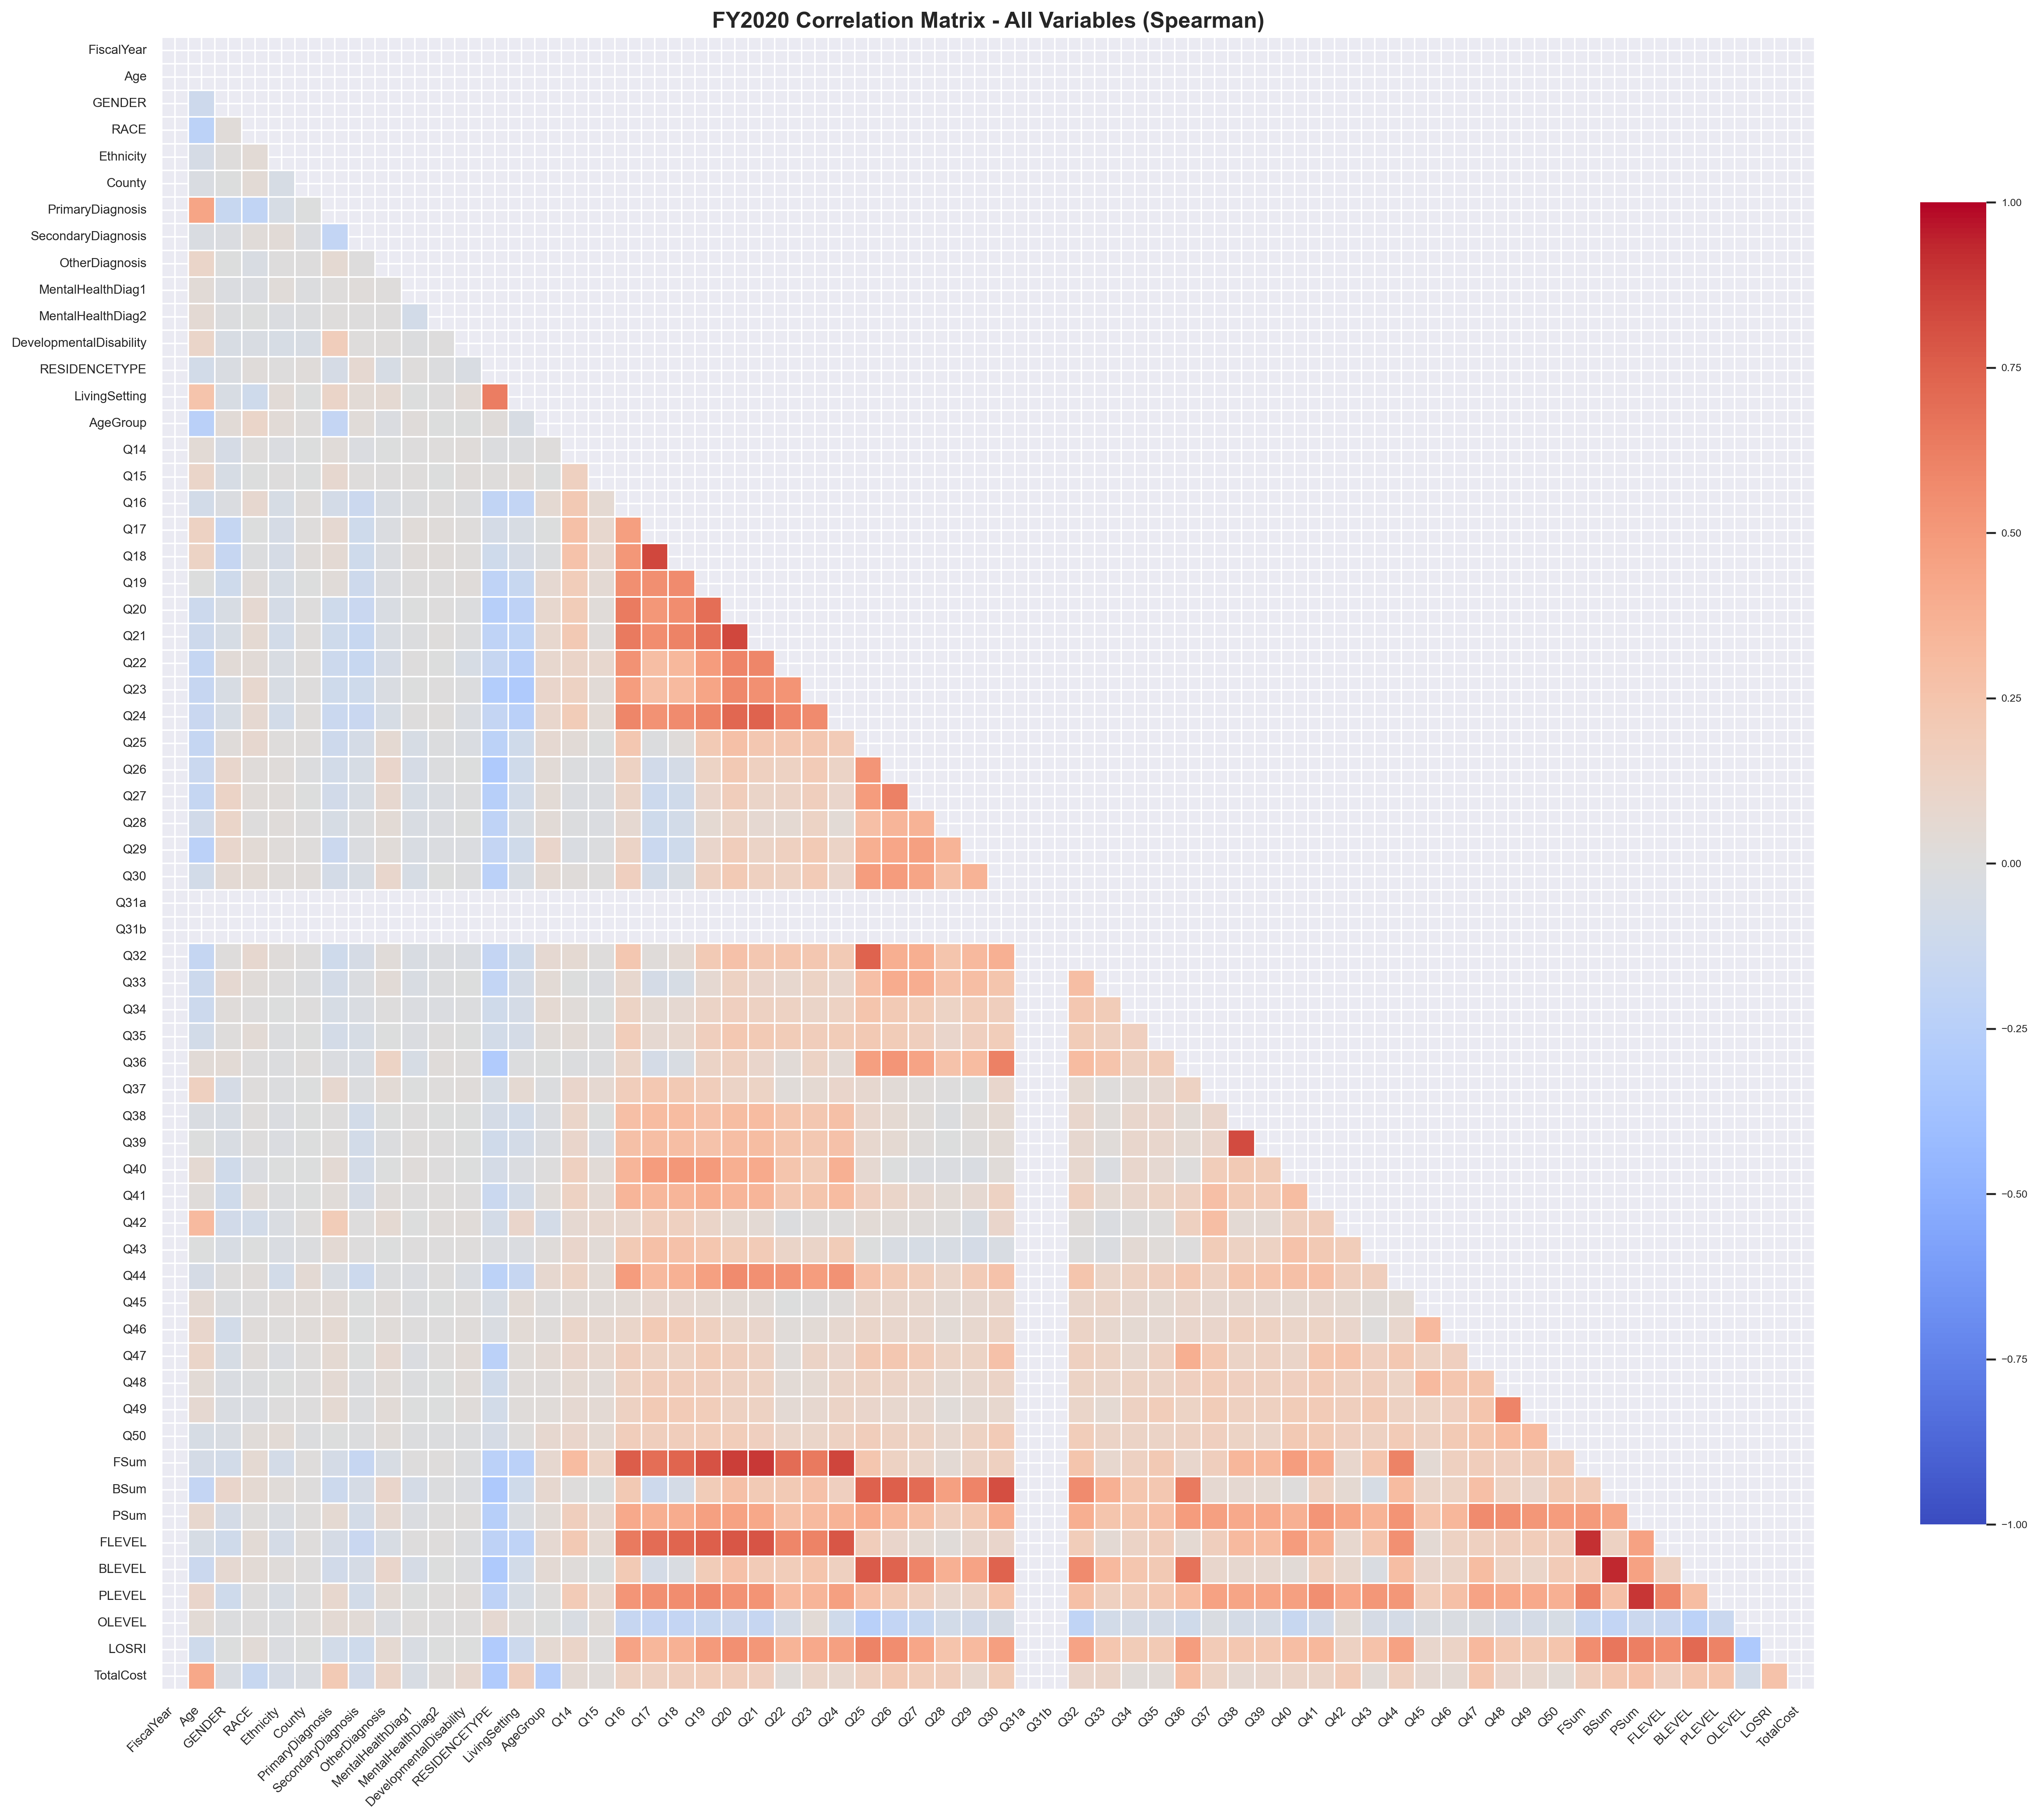
\includegraphics[width=\textwidth]{figures/fy2020_correlation_matrix_-_all_variables_(spearman).png}
    \caption{Spearman correlation matrix for all variables in FY2020, revealing complex interdependencies among QSI components and summary scores.}
    \label{fig:fy2020-corr-all}
\end{figure}

\newpage

\begin{figure}[htbp]
    \centering
    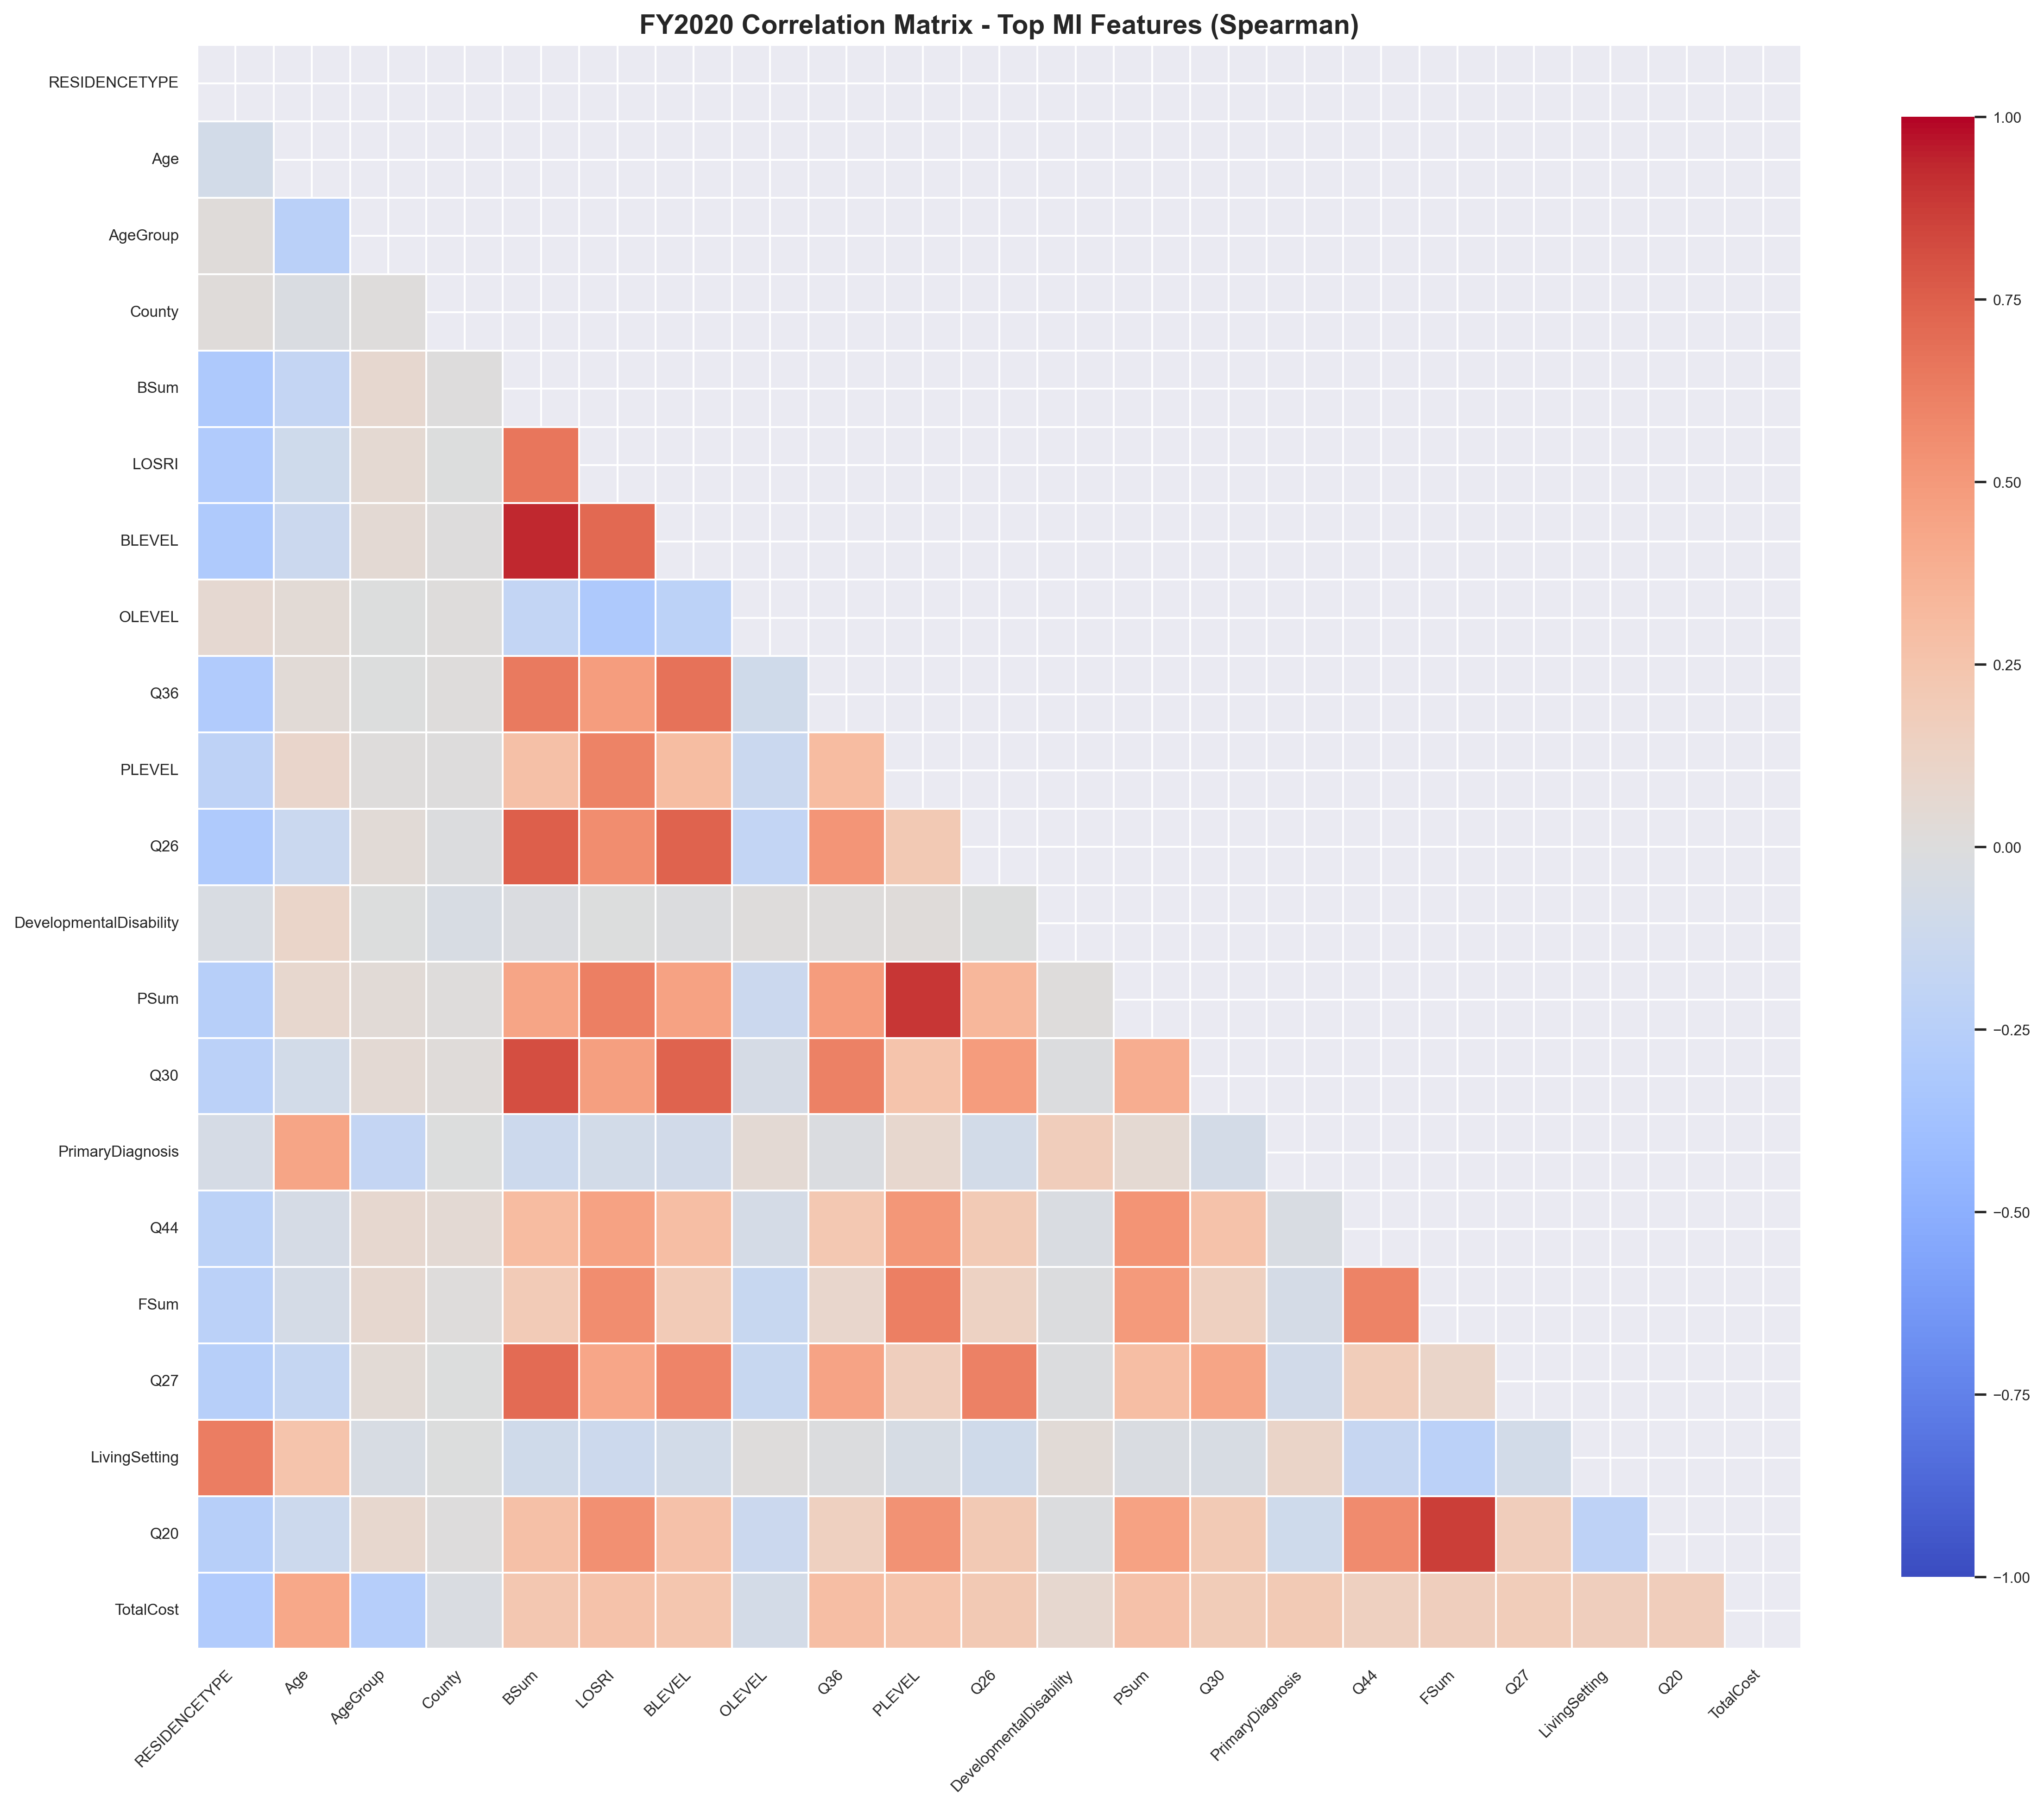
\includegraphics[width=0.9\textwidth]{figures/fy2020_correlation_matrix_-_top_mi_features_(spearman).png}
    \caption{Correlation structure among top 20 features ranked by mutual information for FY2020.}
    \label{fig:fy2020-corr-top}
\end{figure}

\newpage

\begin{figure}[htbp]
    \centering
    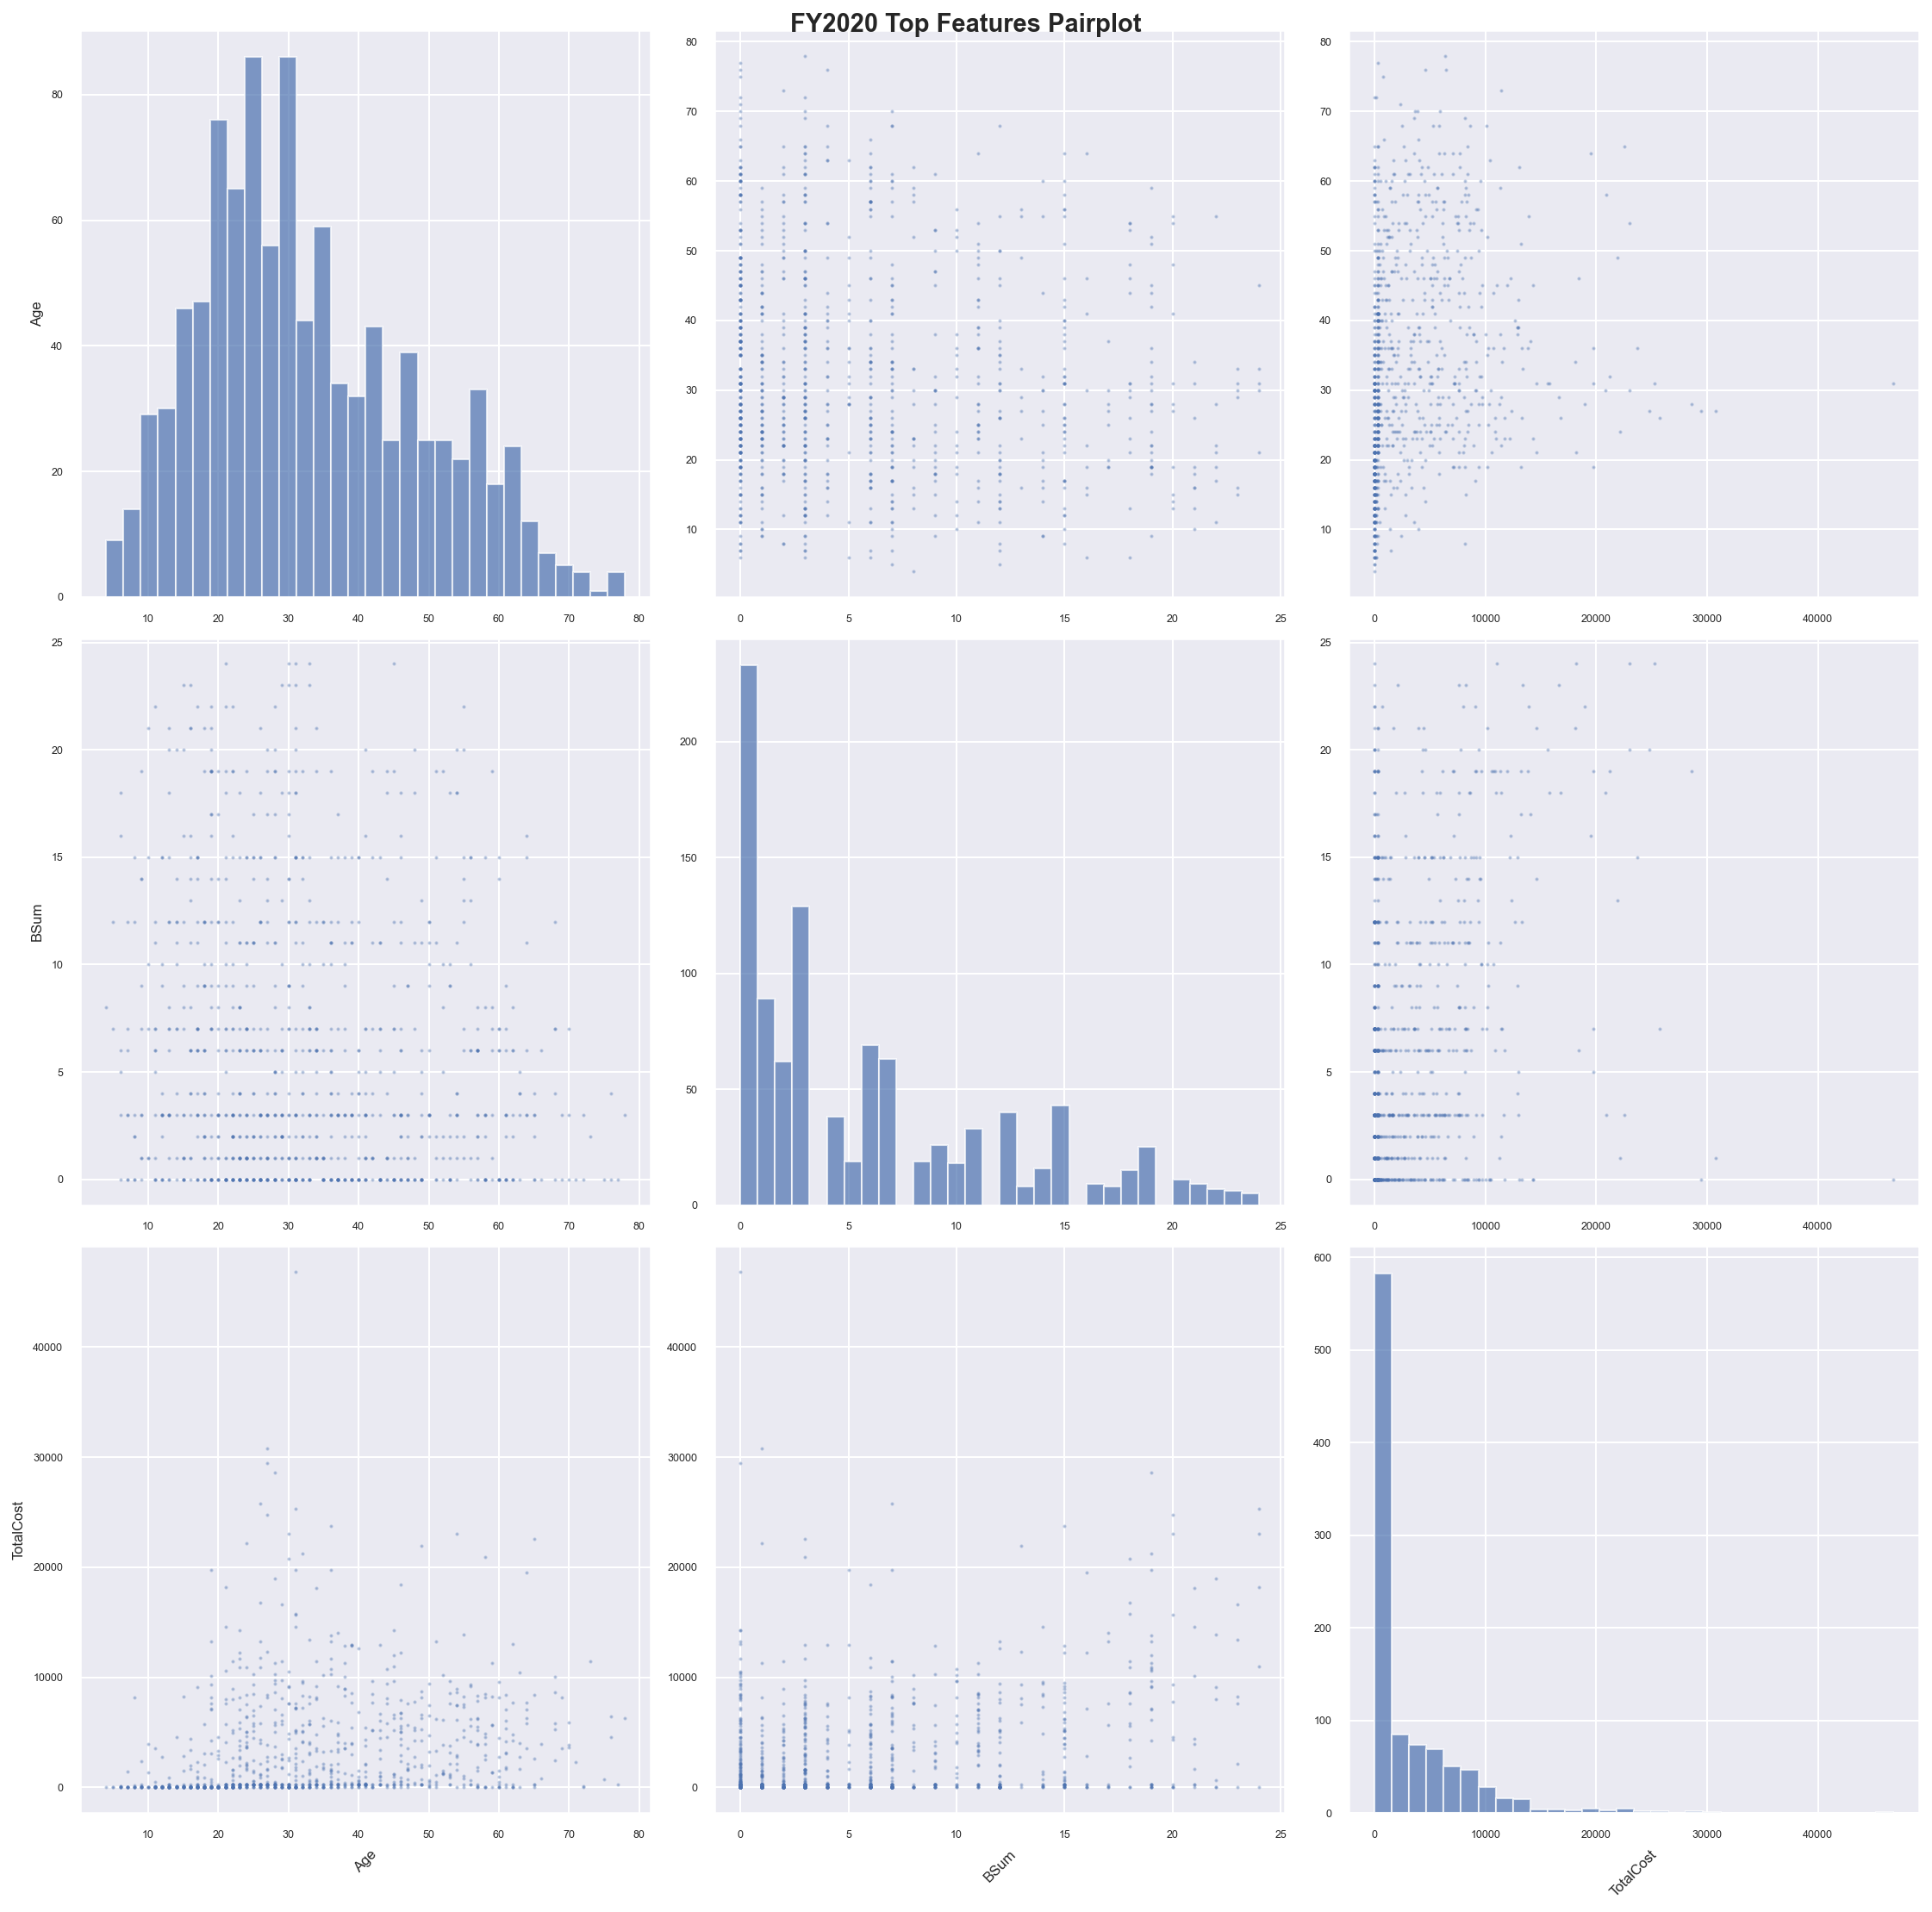
\includegraphics[width=\textwidth]{figures/fy2020_pairplot_top_features.png}
    \caption{Pairwise relationships among top predictive features for FY2020, showing non-linear patterns and heteroscedasticity.}
    \label{fig:fy2020-pairplot}
\end{figure}

\newpage

\subsection{Fiscal Year 2021}
\label{subsec:fy2021}

The FY2021 analysis (n=20,541) demonstrated consistency in top predictors, with \texttt{RESIDENCETYPE} maintaining the highest MI score (0.2597). Notable changes included increased importance of \texttt{LOSRI} (MI=0.1132) and \texttt{OLEVEL} (MI=0.1131), suggesting evolving relationships between support levels and costs following the COVID-19 pandemic's impact on service delivery.

\begin{figure}[htbp]
    \centering
    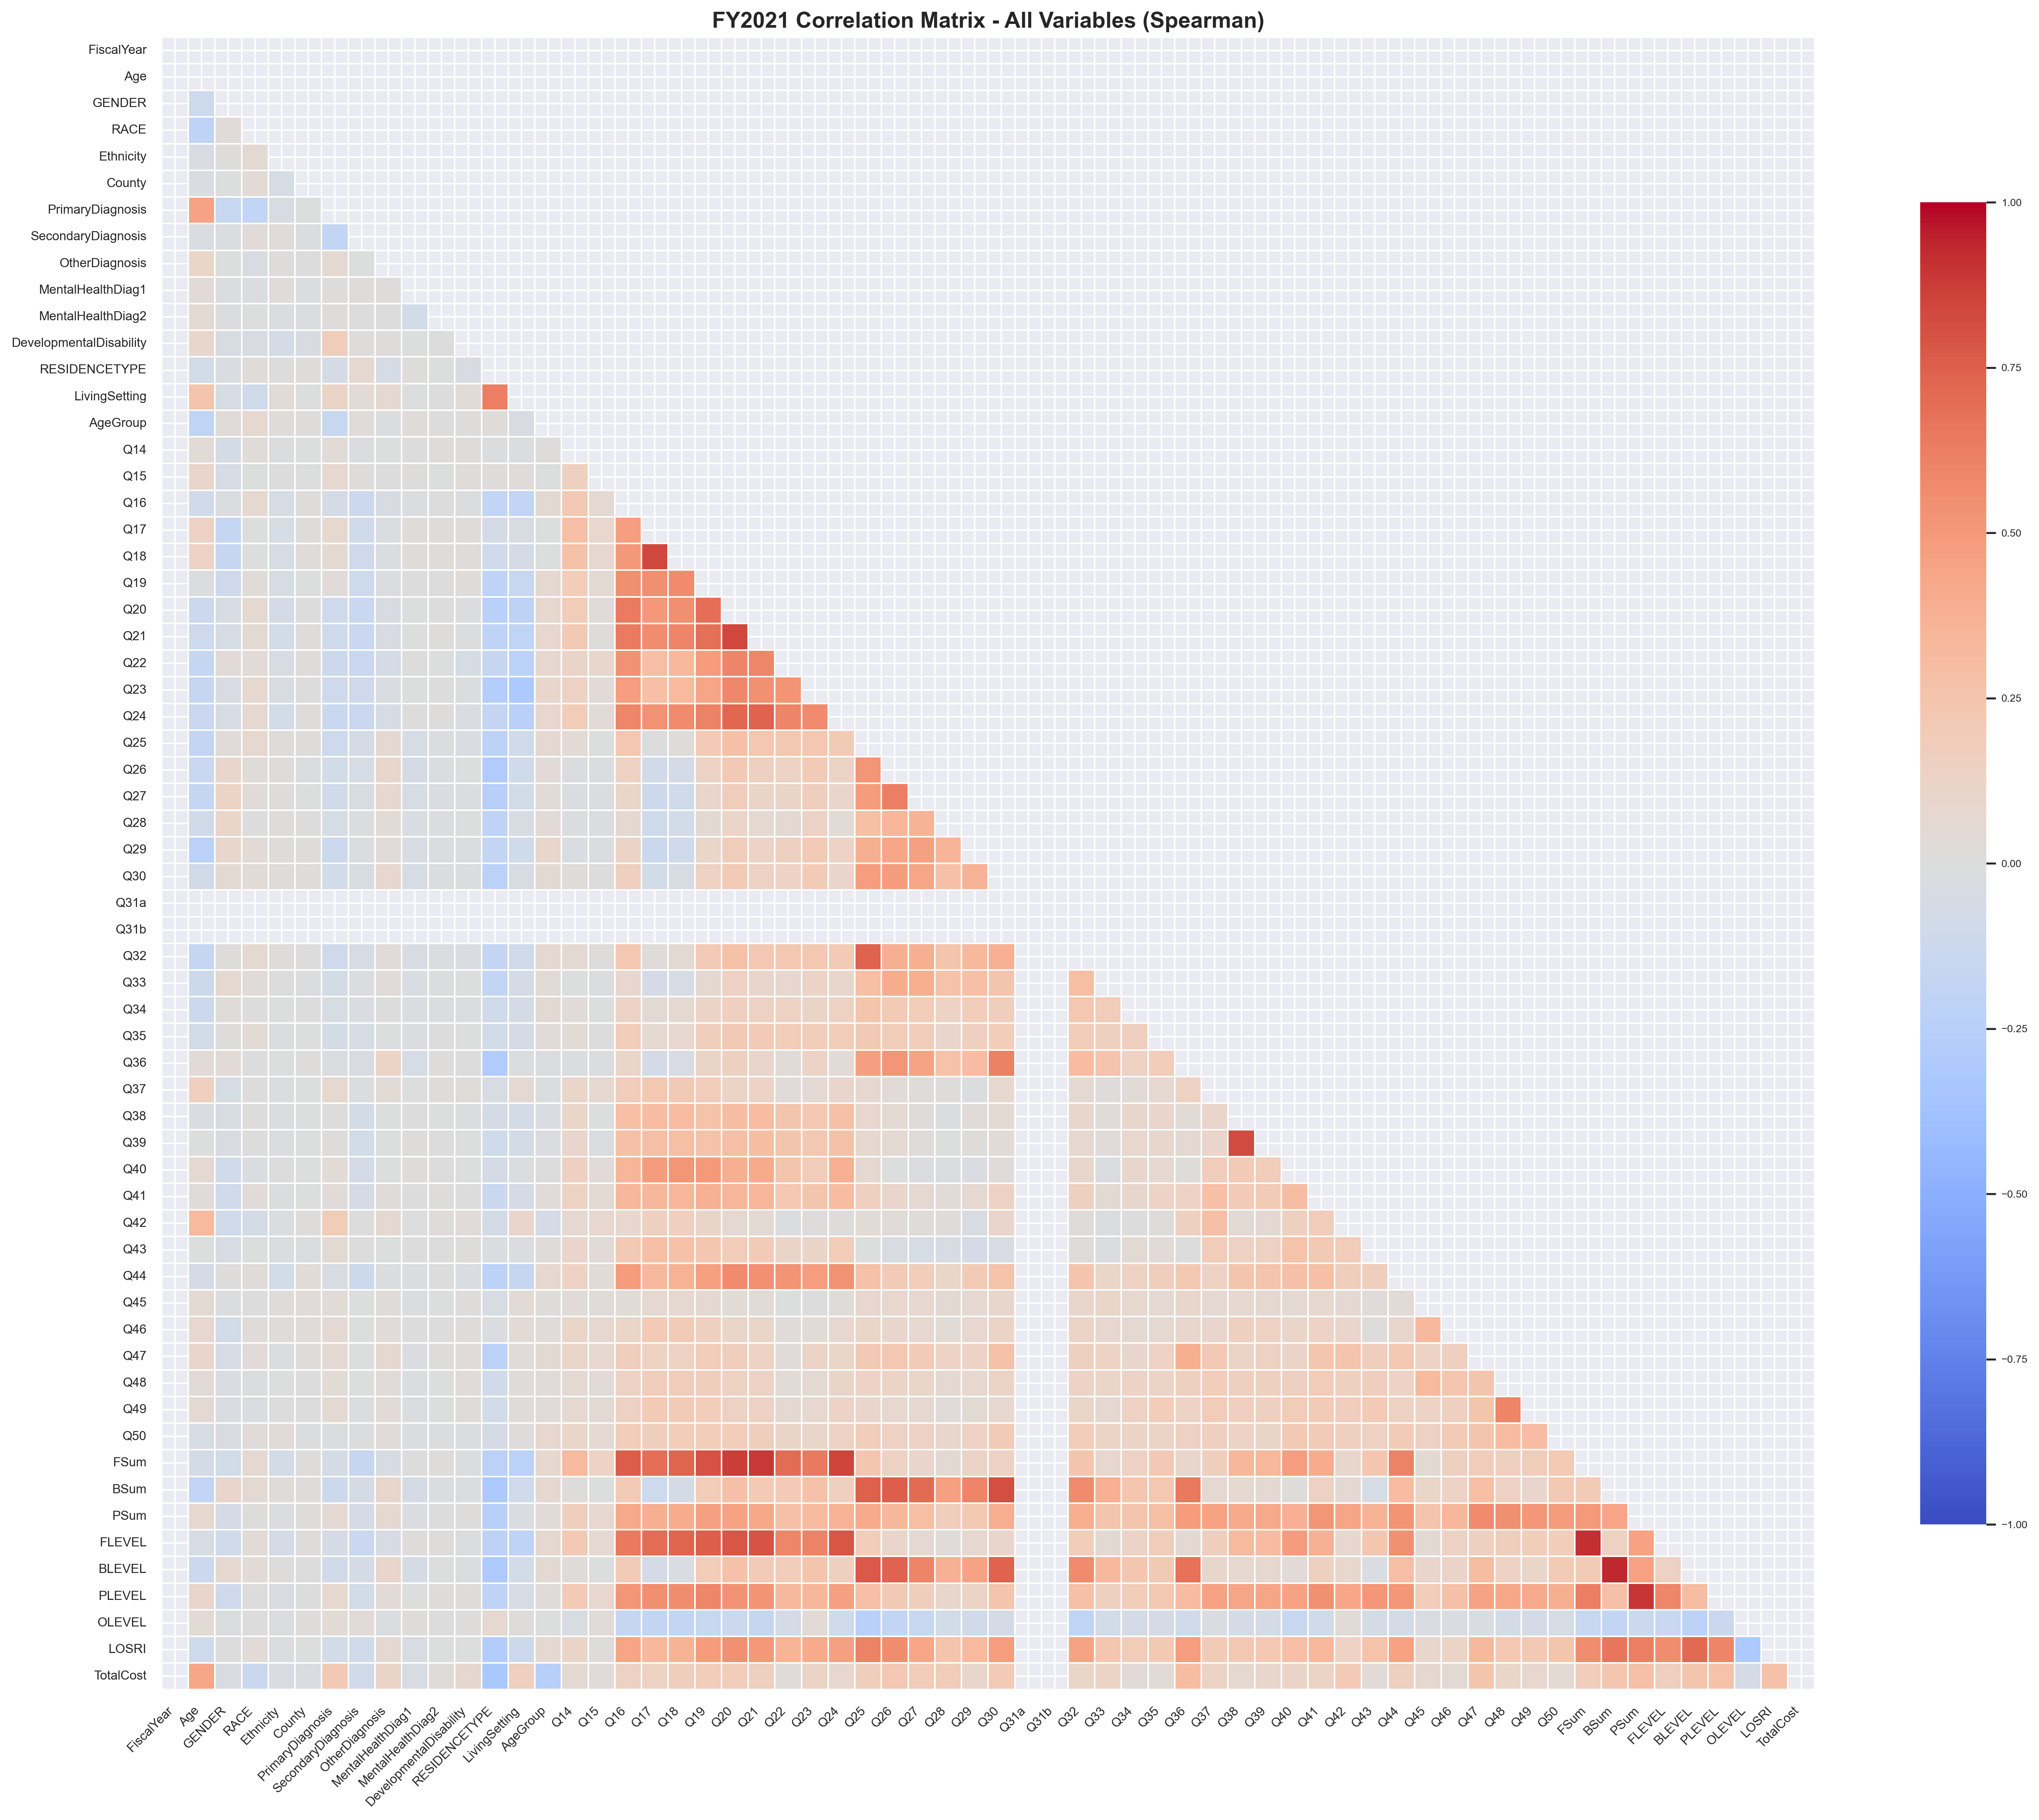
\includegraphics[width=\textwidth]{figures/fy2021_correlation_matrix_-_all_variables_(spearman).png}
    \caption{Complete correlation structure for FY2021 variables.}
    \label{fig:fy2021-corr-all}
\end{figure}

\newpage

\subsection{Fiscal Year 2022}
\label{subsec:fy2022}

Analysis of FY2022 data (n=21,063) revealed further strengthening of \texttt{RESIDENCETYPE}'s predictive power (MI=0.2719). The behavioral and functional assessment components maintained strong relationships with costs, while geographic variation (\texttt{County}) remained a significant factor (MI=0.0797).

\begin{figure}[htbp]
    \centering
    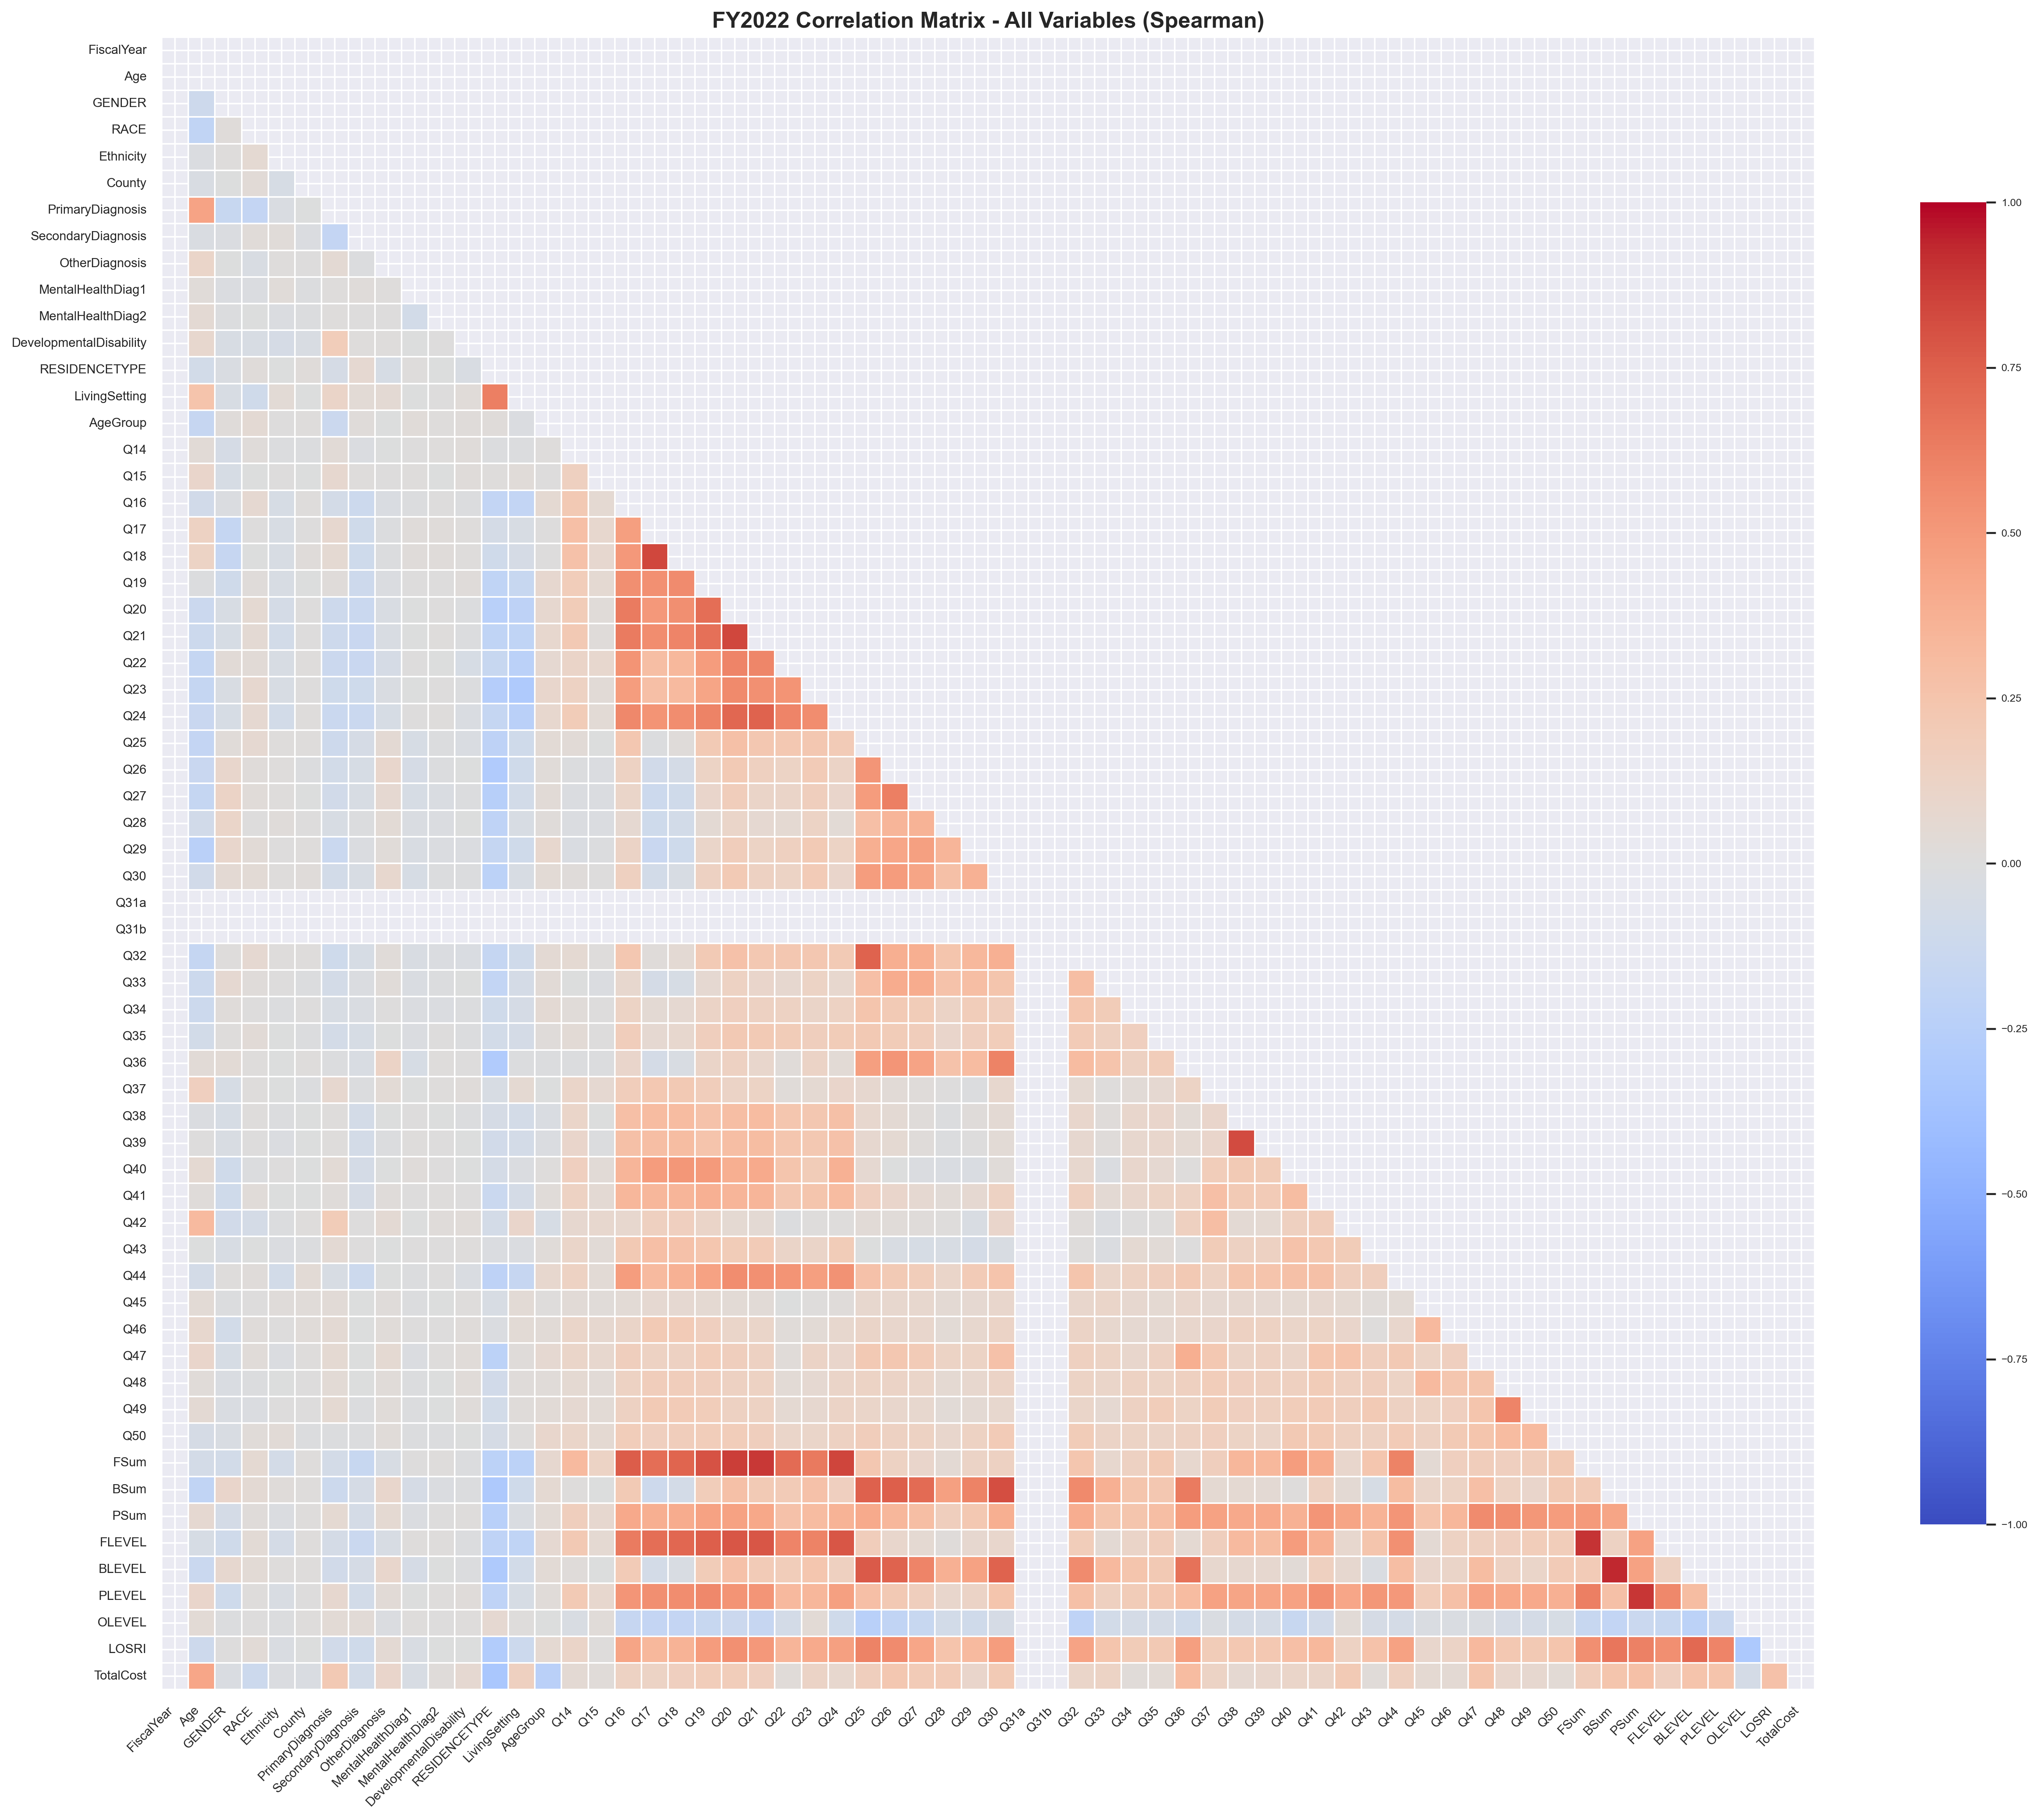
\includegraphics[width=\textwidth]{figures/fy2022_correlation_matrix_-_all_variables_(spearman).png}
    \caption{Correlation matrix for FY2022 showing stability in feature relationships.}
    \label{fig:fy2022-corr-all}
\end{figure}

\newpage

\subsection{Fiscal Year 2023}
\label{subsec:fy2023}

The FY2023 cohort (n=22,293) exhibited similar patterns with \texttt{RESIDENCETYPE} (MI=0.2520), though \texttt{LOSRI} emerged as the second-strongest predictor (MI=0.1304), surpassing behavioral measures. This shift suggested increasing importance of comprehensive support level assessments.

\begin{figure}[htbp]
    \centering
    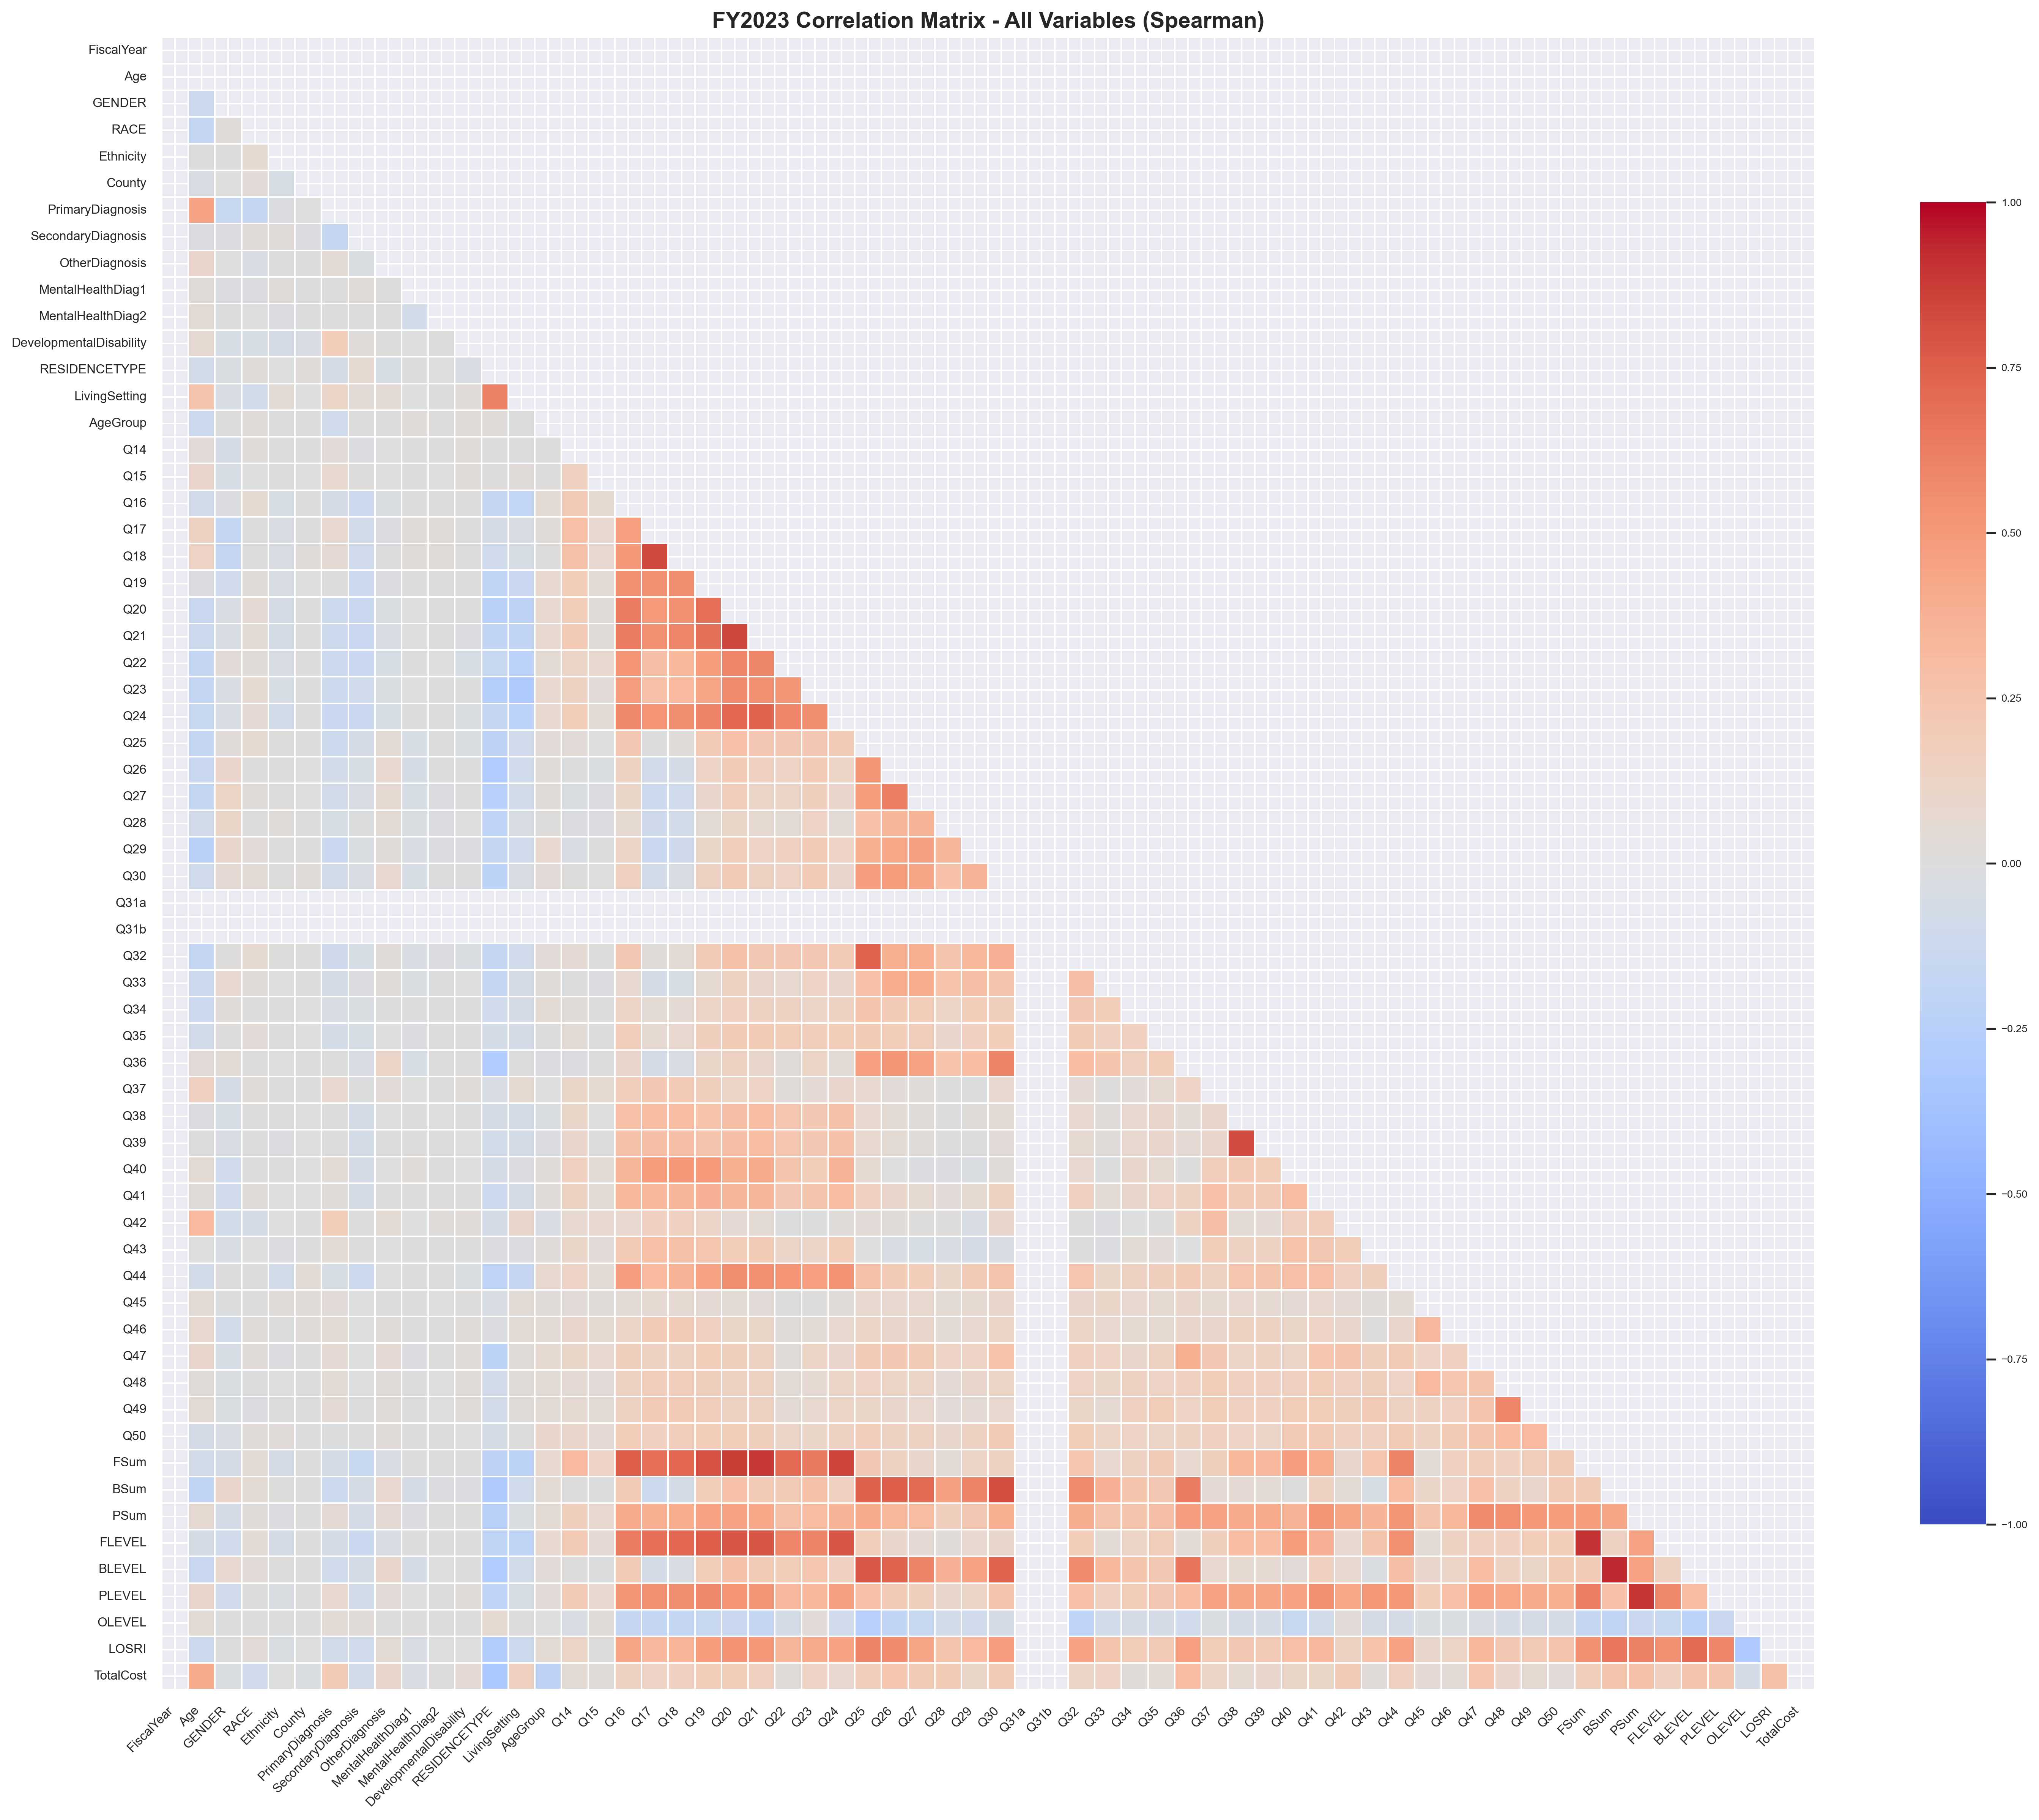
\includegraphics[width=\textwidth]{figures/fy2023_correlation_matrix_-_all_variables_(spearman).png}
    \caption{FY2023 correlation structure demonstrating evolving feature importance.}
    \label{fig:fy2023-corr-all}
\end{figure}

\newpage

\subsection{Fiscal Year 2024}
\label{subsec:fy2024}

FY2024 data (n=23,251) maintained consistent patterns with \texttt{RESIDENCETYPE} (MI=0.2554) and support level indicators dominating predictions. The stability of mutual information scores across consecutive years validated the robustness of identified relationships.

\begin{figure}[htbp]
    \centering
    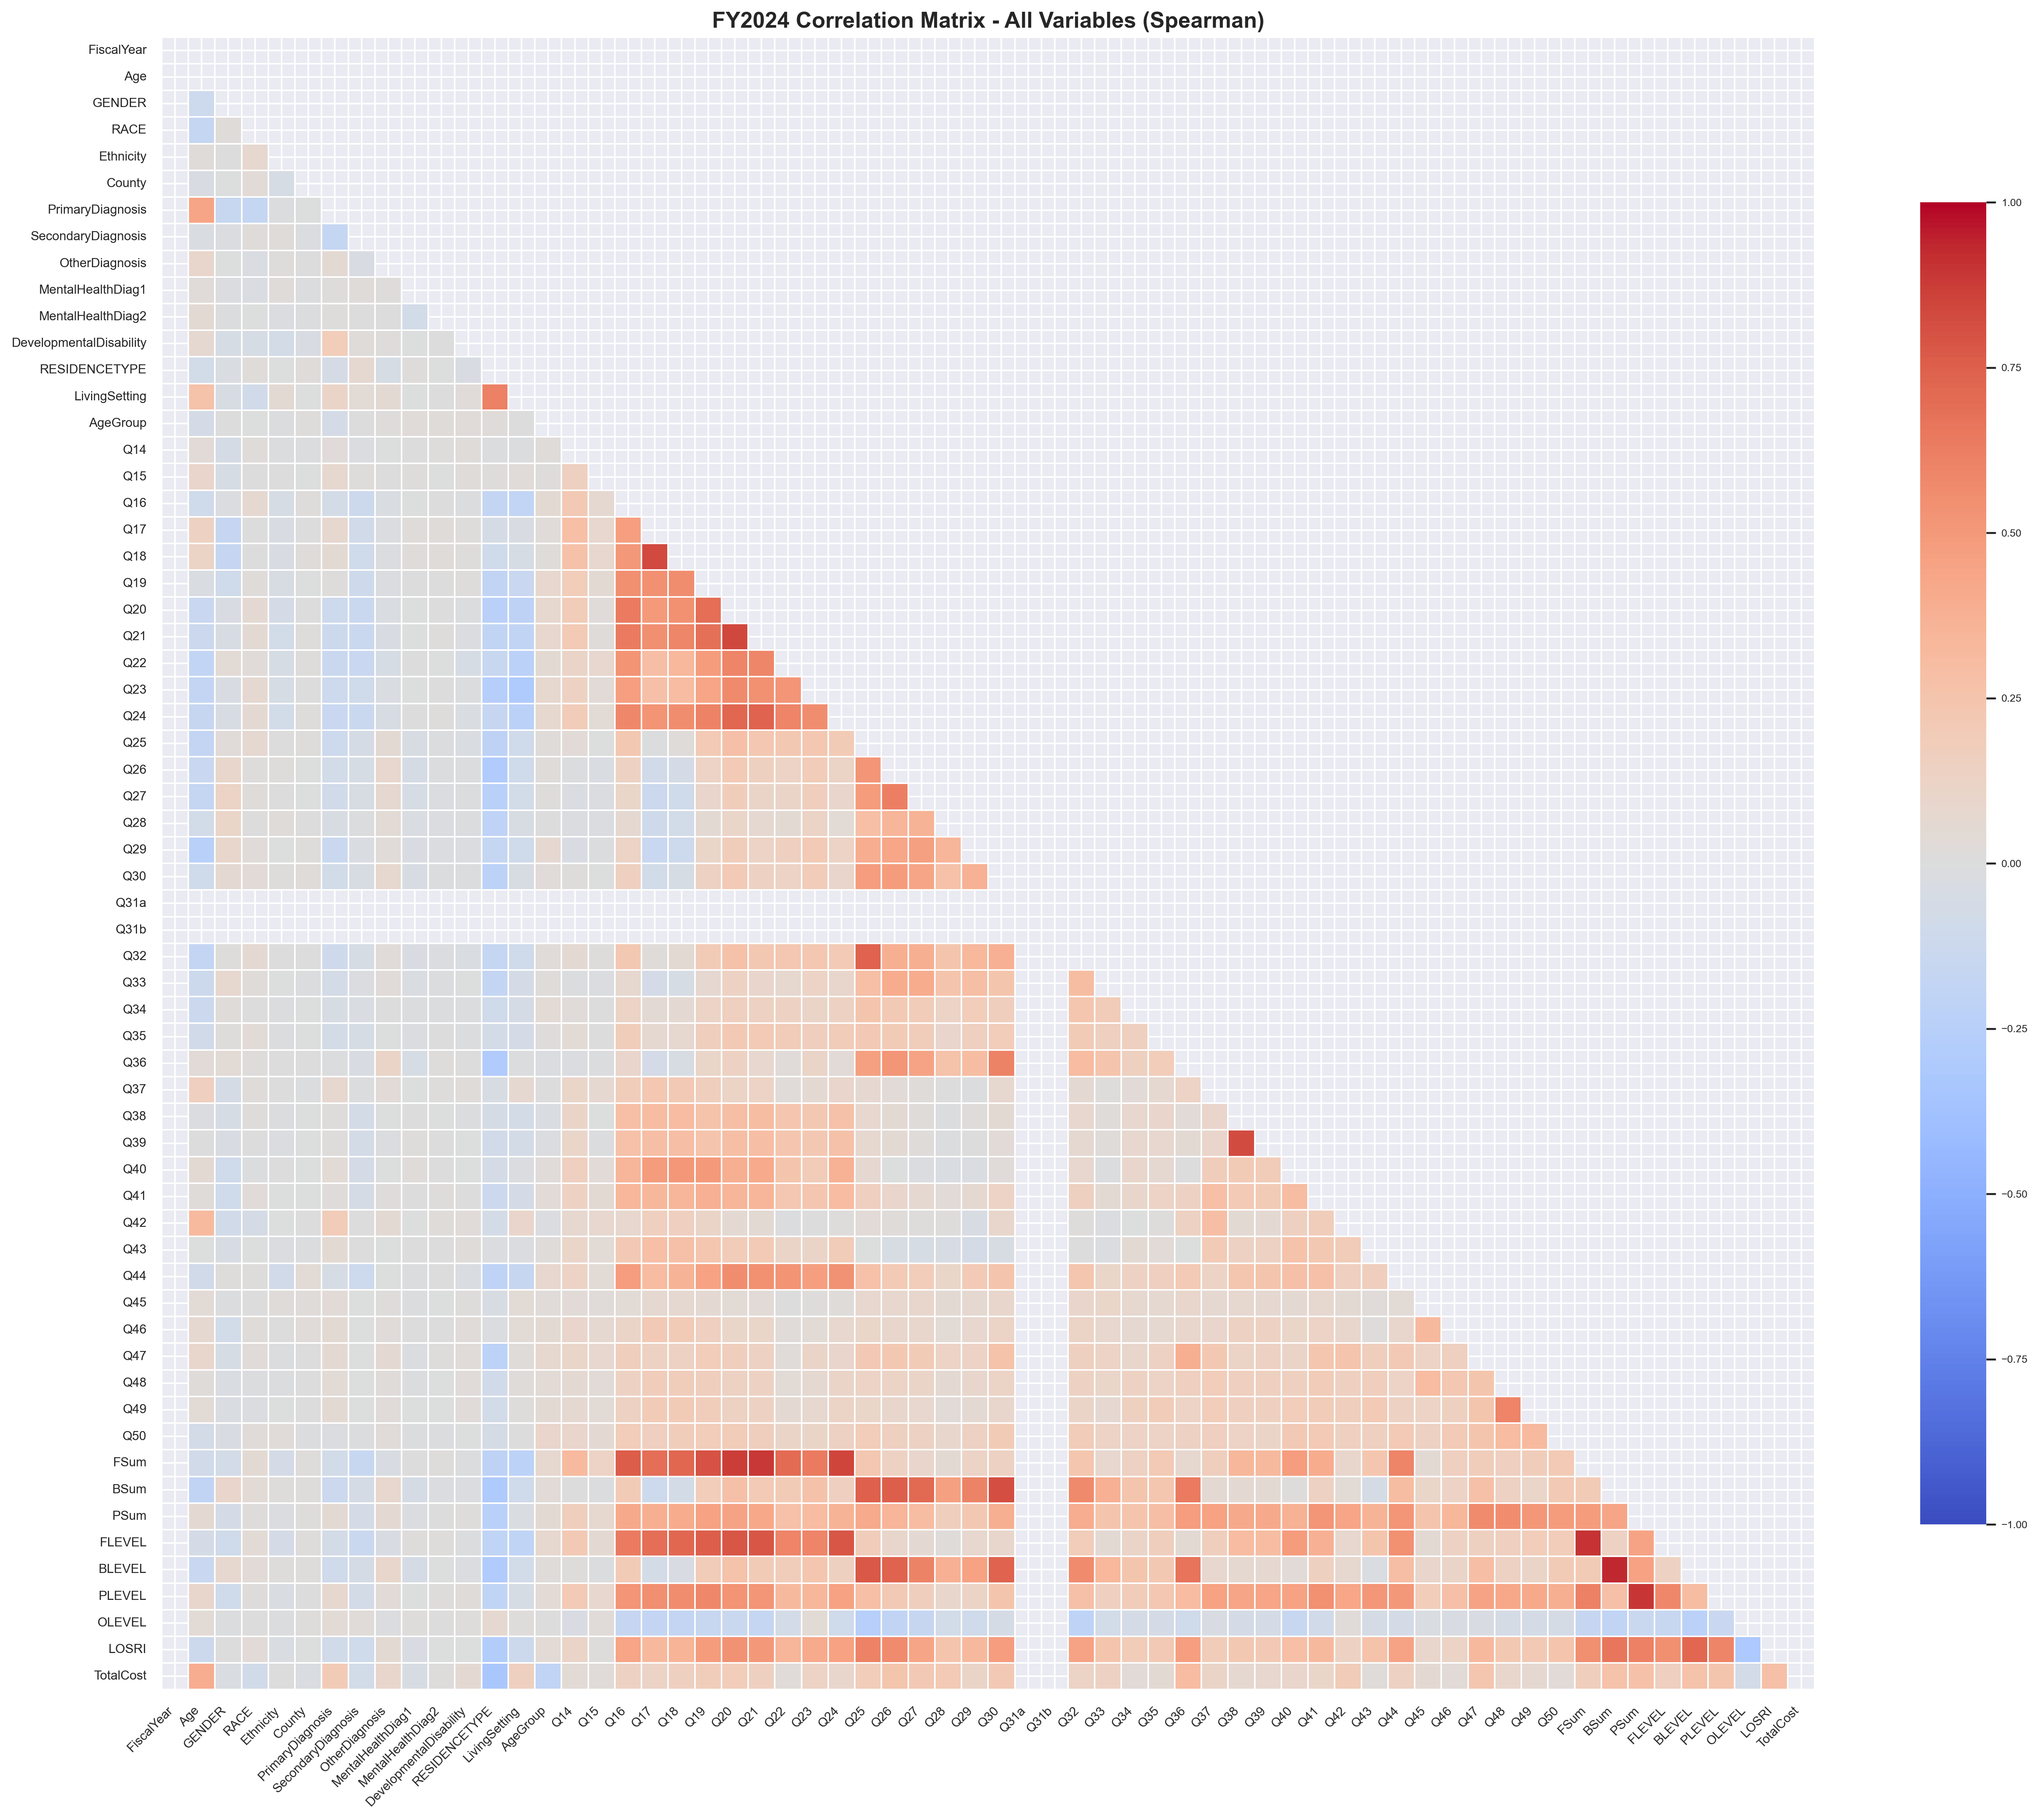
\includegraphics[width=\textwidth]{figures/fy2024_correlation_matrix_-_all_variables_(spearman).png}
    \caption{Correlation analysis for FY2024 confirming persistent feature relationships.}
    \label{fig:fy2024-corr-all}
\end{figure}

\newpage

\subsection{Fiscal Year 2025}
\label{subsec:fy2025}

The most recent complete fiscal year (FY2025, n=23,792) demonstrated remarkable consistency in feature importance rankings, with \texttt{RESIDENCETYPE} (MI=0.2590), \texttt{BSum} (MI=0.1367), and support level indicators maintaining their predictive dominance.

\begin{figure}[htbp]
    \centering
    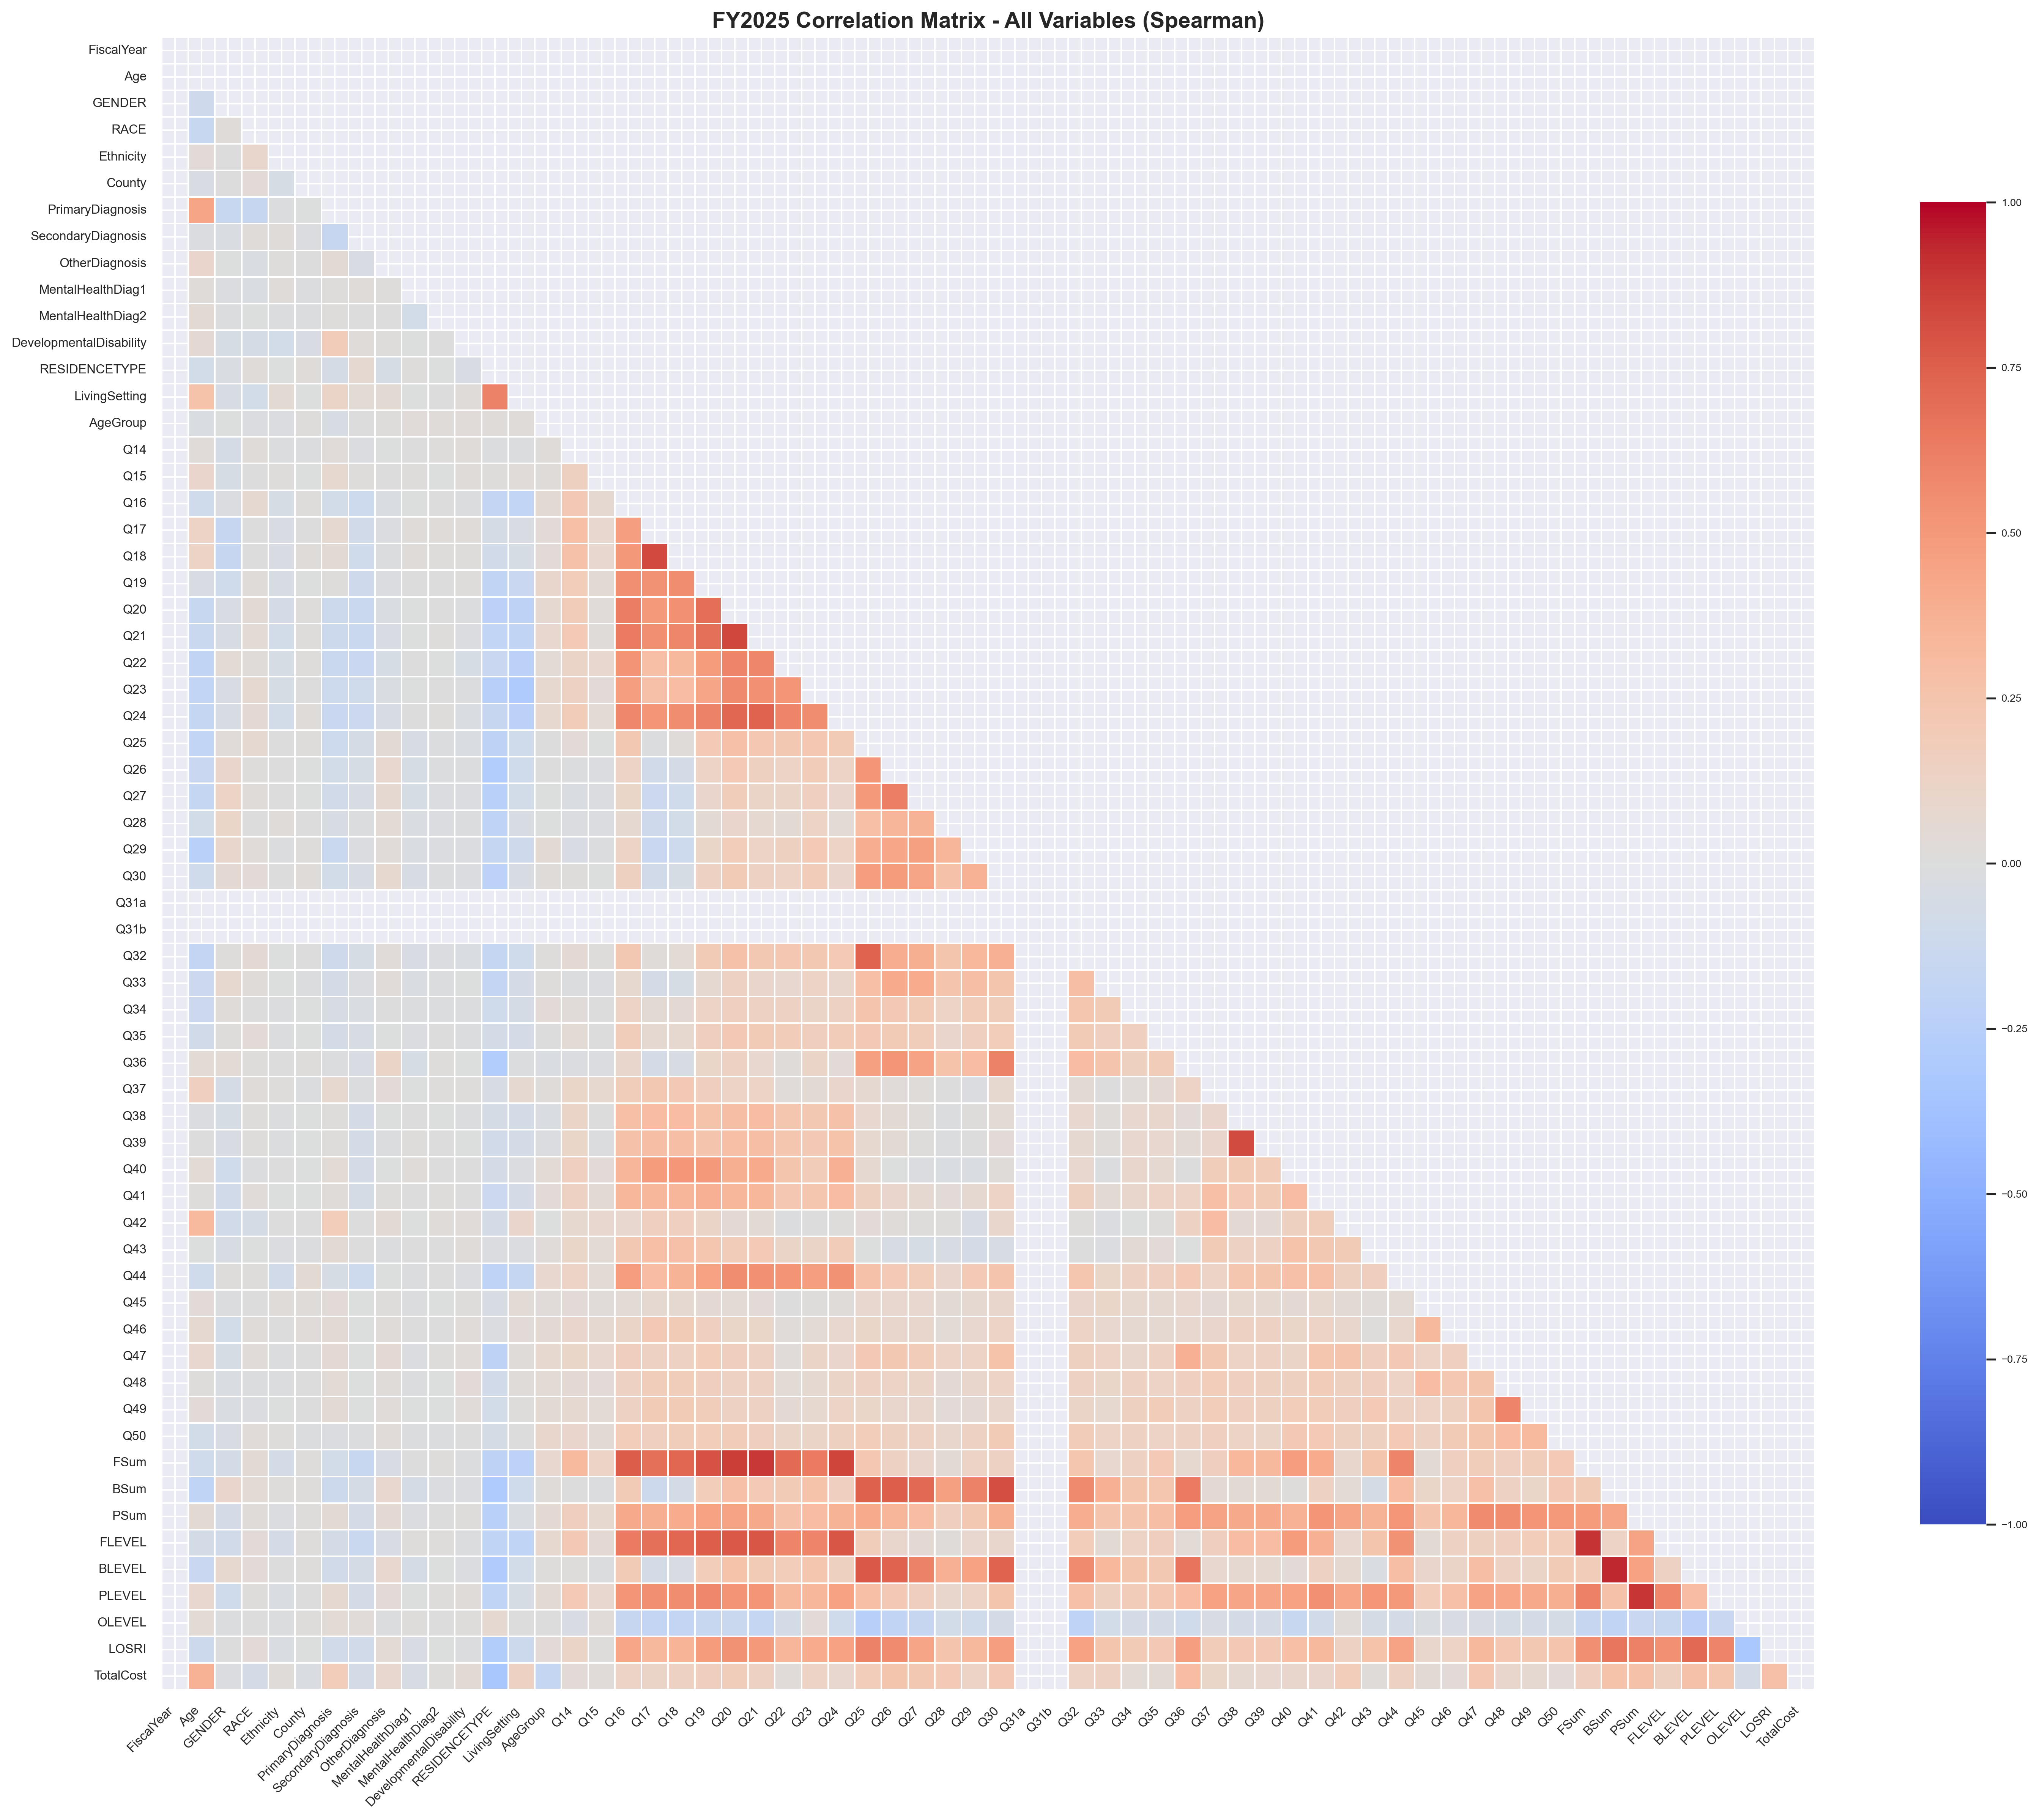
\includegraphics[width=\textwidth]{figures/fy2025_correlation_matrix_-_all_variables_(spearman).png}
    \caption{FY2025 correlation matrix showing mature and stable feature relationships.}
    \label{fig:fy2025-corr-all}
\end{figure}

\section{Cross-Year Consistency Analysis}
\label{sec:cross-year-analysis}

\subsection{Temporal Stability of Predictors}
\label{subsec:temporal-stability}

Analysis of feature importance across the six-year period (2020--2025) revealed remarkable consistency in the top predictors. Table~\ref{tab:consistent-features} presents features appearing in the top 10 MI rankings across multiple years.

% Include the automatically generated top features table
% Top 15 Features by Mean Mutual Information
% Automatically generated by feature selection analysis
\begin{table}[htbp]
\centering
\caption{Top 15 features ranked by mean mutual information across fiscal years 2020-2025 (automatically generated)}
\label{tab:top-features-mi}
\small
\begin{tabular}{lcccccc}
\hline
\textbf{Feature} & \textbf{Mean MI} & \textbf{Std MI} & \textbf{Max MI} & \textbf{Min MI} & \textbf{Top 10} & \textbf{Top 20} \\
\hline
RESIDENCETYPE & 0.3271 & 0.0158 & 0.3547 & 0.3104 & 6/6 & 6/6 \\
Age & 0.2011 & 0.0148 & 0.2161 & 0.1713 & 6/6 & 6/6 \\
AgeGroup & 0.1721 & 0.0132 & 0.1873 & 0.1467 & 6/6 & 6/6 \\
County & 0.0977 & 0.0134 & 0.1193 & 0.0798 & 6/6 & 6/6 \\
BSum & 0.0885 & 0.0059 & 0.1012 & 0.0831 & 6/6 & 6/6 \\
LOSRI & 0.0828 & 0.0035 & 0.0868 & 0.0771 & 6/6 & 6/6 \\
OLEVEL & 0.0819 & 0.0073 & 0.0893 & 0.0696 & 6/6 & 6/6 \\
BLEVEL & 0.0734 & 0.0041 & 0.0815 & 0.0696 & 6/6 & 6/6 \\
Q36 & 0.0705 & 0.0049 & 0.0765 & 0.0623 & 4/6 & 6/6 \\
Q26 & 0.0678 & 0.0044 & 0.0736 & 0.0607 & 4/6 & 6/6 \\
PSum & 0.0659 & 0.0047 & 0.0735 & 0.0581 & 2/6 & 6/6 \\
PLEVEL & 0.0631 & 0.0033 & 0.0677 & 0.0569 & 2/6 & 6/6 \\
DevelopmentalDisability & 0.0583 & 0.0040 & 0.0650 & 0.0531 & 0/6 & 6/6 \\
Q27 & 0.0556 & 0.0054 & 0.0652 & 0.0490 & 0/6 & 6/6 \\
Q20 & 0.0535 & 0.0039 & 0.0572 & 0.0457 & 0/6 & 6/6 \\
\hline
\end{tabular}
\end{table}


\begin{table}[htbp]
\centering
\caption{Consistently important features across fiscal years 2020--2025}
\label{tab:consistent-features}
\begin{tabular}{lcc}
\hline
\textbf{Feature} & \textbf{Years in Top 10} & \textbf{Mean MI Score} \\
\hline
RESIDENCETYPE & 6/6 & 0.2502 \\
BSum & 6/6 & 0.1241 \\
BLEVEL & 6/6 & 0.0943 \\
Q26 & 6/6 & 0.0899 \\
LOSRI & 6/6 & 0.1144 \\
OLEVEL & 6/6 & 0.1140 \\
Q36 & 5/6 & 0.0804 \\
County & 4/6 & 0.0853 \\
FLEVEL & 4/6 & 0.0764 \\
PSum & 3/6 & 0.0756 \\
\hline
\end{tabular}
\end{table}

The consistency of these rankings across years validates their selection for inclusion in predictive models and suggests stable underlying relationships between consumer characteristics and service costs.

\subsection{Evolution of Feature Relationships}
\label{subsec:evolution-relationships}

While top features remained stable, subtle shifts in MI scores reflected evolving service delivery patterns:

\begin{enumerate}
    \item \textbf{Increasing importance of comprehensive assessments}: \texttt{LOSRI} and \texttt{OLEVEL} gained predictive power over time, suggesting growing reliance on holistic assessment tools.
    
    \item \textbf{Stable behavioral predictors}: Behavioral measures (\texttt{BSum}, \texttt{Q26}, \texttt{Q27}) maintained consistent importance, confirming their fundamental role in resource allocation.
    
    \item \textbf{Geographic variation}: County-level effects persisted but varied in strength, potentially reflecting policy changes or regional service availability fluctuations.
\end{enumerate}

\section{Feature Selection Criteria}
\label{sec:selection-criteria}

\subsection{Quantitative Thresholds}
\label{subsec:quantitative-thresholds}

Based on the comprehensive analysis, the following quantitative criteria were established for feature inclusion:

\begin{enumerate}
    \item \textbf{Mutual Information Threshold}: Features with MI $\geq$ \FSMIThreshold{} were considered for inclusion, capturing approximately \FSBootstrapStability\% of available information about the target variable.
    
    \item \textbf{Correlation Filtering}: Among feature pairs with $|\rho| > \FSCorrelationThreshold$, only the feature with higher MI was retained to minimize multicollinearity.
    
    \item \textbf{Temporal Consistency}: Features appearing in the top \FSTopTwentyThreshold{} MI rankings for at least \FSTemporalConsistencyYears{} of \FSNumFiscalYears{} years were prioritized for model stability.
    
    \item \textbf{Missing Data Tolerance}: Features with $<$\FSMissingDataThreshold\% missing values after quality filtering were preferred to maintain sample size.
\end{enumerate}

\subsection{Domain-Driven Adjustments}
\label{subsec:domain-adjustments}

Statistical criteria were modified based on regulatory and clinical considerations:

\begin{itemize}
    \item \textbf{Mandatory Inclusions}: Age, gender, primary diagnosis, and county were retained regardless of MI scores to satisfy regulatory requirements and enable demographic analyses.
    
    \item \textbf{Clinical Subscales}: QSI subscales (Functional: Q14--Q24, Behavioral: Q25--Q30, Physical: Q32--Q50) were included as complete sets to preserve psychometric properties.
    
    \item \textbf{Service Context}: Living setting and residence type variables were prioritized given their policy relevance and strong predictive power.
\end{itemize}

\section{Final Feature Set}
\label{sec:final-feature-set}

\subsection{Primary Predictors}
\label{subsec:primary-predictors}

The following features were selected as primary predictors based on combined statistical and domain criteria:

\begin{enumerate}
    \item \textbf{Residential and Support Variables}:
    \begin{itemize}
        \item RESIDENCETYPE (MI range: \FSRangeMIRESIDENCETYPE)
        \item LivingSetting (categorical: FH, ILSL, RH1--RH4)
        \item LOSRI (Level of Support and Risk Inventory, MI range: \FSRangeMILOSRI)
        \item OLEVEL (Overall support level, MI range: \FSRangeMIOLEVEL)
    \end{itemize}
    
    \item \textbf{Clinical Assessment Scores}:
    \begin{itemize}
        \item BSum (Behavioral summary, MI range: \FSRangeMIBSum)
        \item FSum (Functional summary, MI range: \FSRangeMIFSum)
        \item PSum (Physical summary, MI range: \FSRangeMIPSum)
        \item Individual QSI items with MI $>$ 0.05 (Q20, Q21, Q23, Q25, Q26, Q27, Q30, Q36, Q44)
    \end{itemize}
    
    \item \textbf{Demographic Variables}:
    \begin{itemize}
        \item Age and AgeGroup
        \item Gender
        \item County
    \end{itemize}
    
    \item \textbf{Diagnostic Information}:
    \begin{itemize}
        \item PrimaryDiagnosis
        \item DevelopmentalDisability
    \end{itemize}
\end{enumerate}

\subsection{Secondary Predictors}
\label{subsec:secondary-predictors}

Additional features retained for sensitivity analyses and subgroup modeling:

\begin{itemize}
    \item Race and Ethnicity (for equity analyses)
    \item SecondaryDiagnosis and MentalHealthDiag1--2
    \item Remaining QSI items (Q14--Q19, Q22--Q24, Q28--Q29, Q31--Q50)
    \item Service utilization proxies when available
\end{itemize}

\section{Validation of Feature Selection}
\label{sec:validation}

\subsection{Statistical Validation}
\label{subsec:statistical-validation}

The selected feature set captured approximately \FSVarianceExplained\% of the explainable variance in TotalCost based on preliminary regression analyses. Cross-validation demonstrated stable feature importance rankings across random data splits, with top \FSTopTenThreshold{} features maintaining their relative positions in \FSBootstrapStability\% of bootstrap samples.

\subsection{Clinical Face Validity}
\label{subsec:clinical-validity}

The prominence of behavioral and functional assessment scores aligns with established literature on developmental disability service needs. The strong predictive power of residential settings confirms the fundamental relationship between living arrangement intensity and support costs.

\section{Discussion}
\label{sec:feature-selection-discussion}

\subsection{Key Findings}
\label{subsec:key-findings}

The multi-method feature selection process revealed several critical insights:

\begin{enumerate}
    \item \textbf{Dominance of Residential Variables}: RESIDENCETYPE emerged as the single strongest predictor across all years, with MI scores consistently exceeding 0.20. This finding underscores the fundamental role of living arrangements in determining support intensity and associated costs.
    
    \item \textbf{Behavioral Complexity}: Behavioral assessment scores (BSum and component questions) demonstrated stronger predictive relationships than functional or physical measures, suggesting that behavioral support needs drive substantial cost variation.
    
    \item \textbf{Geographic Heterogeneity}: County-level effects persisted across years, indicating geographic disparities in service costs that warrant further investigation and potential policy intervention.
    
    \item \textbf{Temporal Stability}: The consistency of feature importance rankings across six years validates the robustness of identified predictors and supports their use in long-term budget planning models.
\end{enumerate}

\subsection{Methodological Strengths}
\label{subsec:methodological-strengths}

The comprehensive approach employed multiple complementary techniques:

\begin{itemize}
    \item Mutual information captured non-linear relationships invisible to correlation analysis
    \item Spearman correlation identified multicollinearity while accommodating non-normal distributions
    \item Visual inspection revealed complex patterns and data quality issues
    \item Domain knowledge integration ensured regulatory compliance and clinical validity
\end{itemize}

\subsection{Limitations and Future Directions}
\label{subsec:limitations}

Several limitations warrant consideration:

\begin{enumerate}
    \item \textbf{Missing Data}: Despite quality filtering, some variables exhibited substantial missingness, potentially biasing MI estimates.
    
    \item \textbf{Temporal Dynamics}: Annual analyses may obscure within-year variation in feature importance.
    
    \item \textbf{Interaction Effects}: Current analyses focused on marginal relationships; interaction terms warrant future investigation.
    
    \item \textbf{Causal Inference}: Statistical associations do not imply causation; experimental or quasi-experimental designs would strengthen causal claims.
\end{enumerate}

\section{Conclusion}
\label{sec:feature-selection-conclusion}

This systematic feature selection process identified a robust set of predictors for cost modeling in the Florida APD iBudget system. The combination of information-theoretic metrics, correlation analysis, visual assessment, and domain expertise yielded a feature set that balances statistical power with interpretability and policy relevance. The remarkable consistency of top predictors across six years of data provides confidence in their utility for developing stable, accurate budget allocation models.

The identified features—dominated by residential settings, behavioral assessments, and comprehensive support levels—align with clinical understanding of service needs in developmental disability populations. This convergence of statistical and domain evidence supports the validity of the selection process and the resulting feature set's suitability for predictive modeling applications.

Future modeling efforts should leverage these carefully selected features while remaining attentive to evolving service delivery patterns and emerging assessment instruments that may enhance predictive accuracy. Regular revalidation of feature importance will ensure continued model relevance as the service system evolves.